\chapter{Localization system evaluation} \label{chap:localization-system-evaluation}



\section*{}

This chapter presents several test scenarios that were devised to evaluate the implemented localization system. They aim to test the accuracy and robustness of the implementation under different environmental conditions and hardware configurations.



\section{Testing platforms}

The localization system was tested on laser sensor data retrieved from three different mobile robot platforms and executed on the same computer in order to allow a direct comparison of computation time. This computer was a Clevo P370EM3 laptop (with a Intel Core i7 3630QM CPU at 2.4GHz, 16 GB of RAM DDR3, NVidia GTX680M graphics card and a Samsung 840 Pro SSD) and it was running Ubuntu 12.04 along with \gls{ros} Hydro, \gls{pcl} 1.7 and Gazebo 1.9.

The sensor data was recorded into rosbags, and is publicly available at\footnote{\url{https://github.com/carlosmccosta/dynamic_robot_localization_tests}} along with all the detailed results and experiments videos, in order to allow future comparisons with other localization systems. The hardware specifications of the \glspl{lidar} used is presented in \cref{tab:localization-system-evaluation_laser-hardware-specifications} and the laser points after downsampling and registration can be seen on the movement paths figures as green circles (inliers) and red circles (outliers).


\subsection{Jarvis platform}

The Jarvis platform is an autonomous ground vehicle equipped with a SICK NAV 350 laser for self-localization (mounted about 2 meters from the floor) and a SICK S3000 laser for collision avoidance (mounted about 0.20 meters from the floor). It uses a tricycle locomotion system with two back wheels and a steerable wheel at the front. In \cref{fig:localization-system-evaluation_jarvis} the robot is performing a delivery task with the package on top of a moving support. The 3 \gls{dof} ground truth was provided by the SICK NAV350 system and relied on 6 laser reflectors (with 9 cm of diameter) to perform the pose estimations (it is certified for robot docking operations with precision up to 4 millimeters).

\begin{figure}[H]
	\centering
	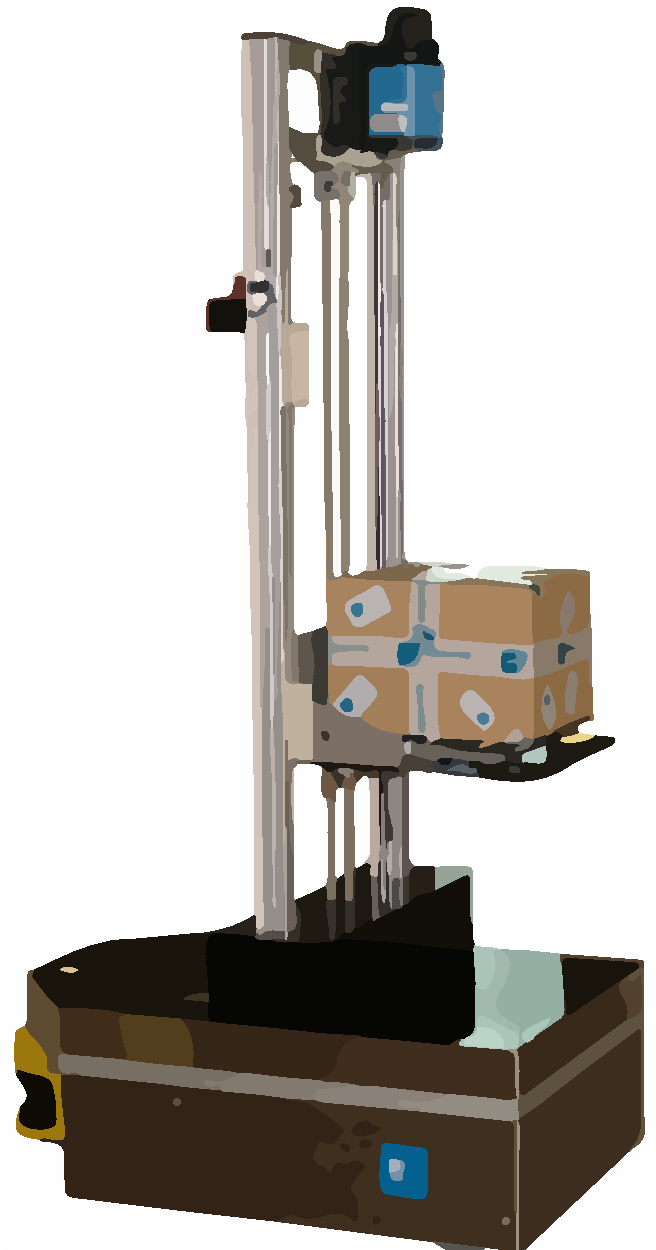
\includegraphics[width=0.28\textwidth]{localization-system-evaluation/testing-platforms/jarvis}
	\caption{Jarvis testing platform}
	\label{fig:localization-system-evaluation_jarvis}
\end{figure}


\subsection{Pioneer 3-DX platform}

The Pioneer 3-DX shown in \cref{fig:localization-system-evaluation_pioneer} is a small lightweight robot equipped with a SICK LMS-200 laser (mounted about 48 cm from the floor) and a Kinect (mounted about 78 cm from the floor). It uses a two-wheel two-motor differential drive locomotion system and can reach a linear speed of 1.2 m/s and angular velocity of 300º/s. The 3 \gls{dof} ground truth was provided by 8 Raptor-E cameras \footnote{\url{http://www.motionanalysis.com/html/movement/raptore.html}} and according to \cite{Sturm2012} it had less than 1 cm in translation error and less than 0.5 degrees in rotation error.

\begin{figure}[H]
	\centering
	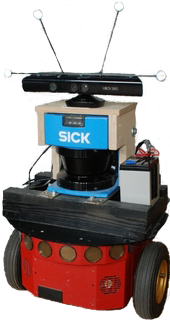
\includegraphics[width=0.25\textwidth]{localization-system-evaluation/testing-platforms/pioneer-3dx}
	\caption{Pioneer 3-DX testing platform}
	\label{fig:localization-system-evaluation_pioneer}
\end{figure}


\subsection{Guardian platform}

The Guardian platform is an autonomous mobile manipulator equipped with a Hokuyo URG-04LX laser in the front and a Hokuyo URG-04LX\_UG01 laser in the back (both mounted about 0.37 meters from the ground). The front laser had a tilting platform which allows 3D mapping of the environment. The arm is a SCHUNK Powerball LWA 4P and in \cref{fig:localization-system-evaluation_guardian} it is attached to a stud welding machine (in simulation it is attached to a video projector). It uses a differential drive locomotion system and can be moved with wheels or with tracks. This platform didn't have a certified ground truth and as such, the results could not be quantified with an external localization system (the results performed with the Gazebo simulator will be presented instead - robot model shown in \cref{fig:localization-system-evaluation_guardian_gazebo}).

\begin{figure}[H]
	\centering
	\begin{minipage}[h]{0.497\textwidth}
		\centering
		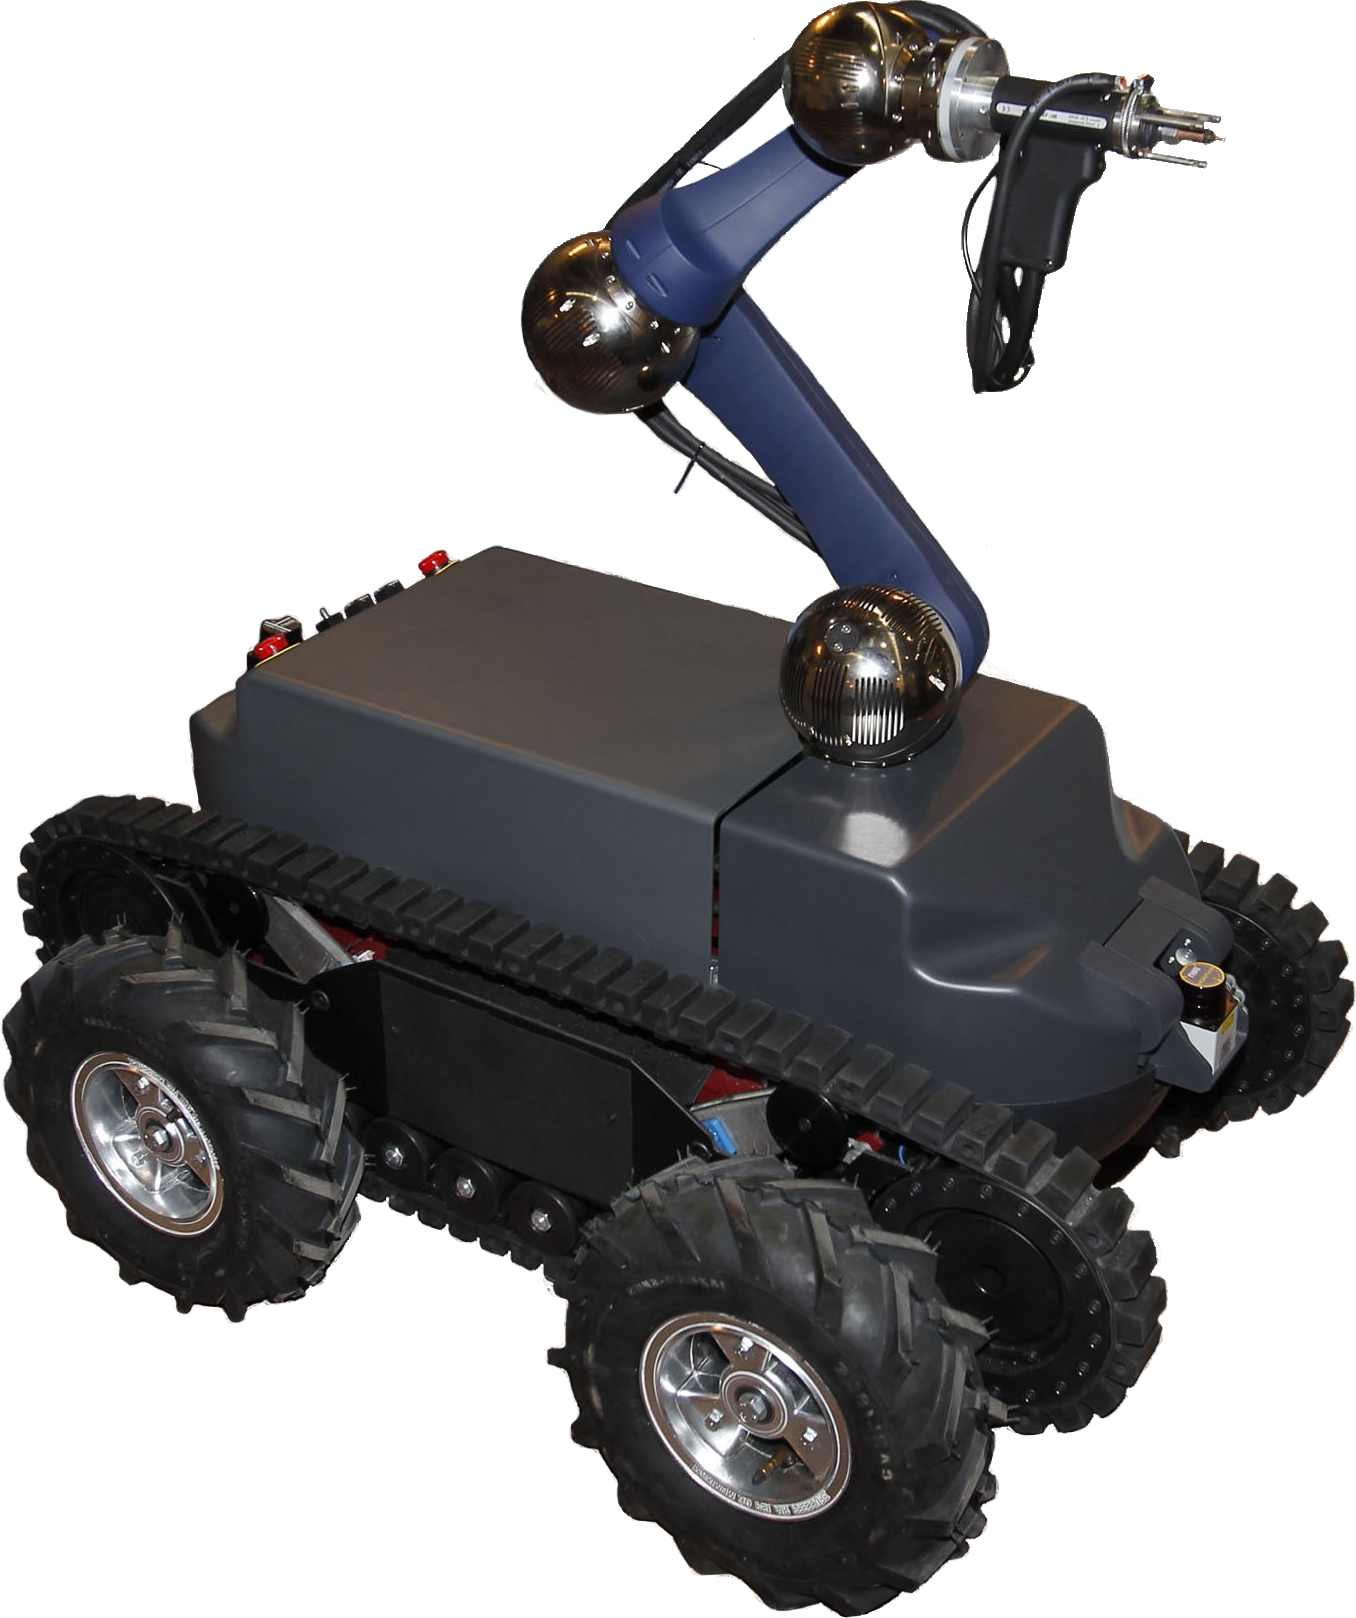
\includegraphics[width=0.7\textwidth]{localization-system-evaluation/testing-platforms/guardian}
		\caption{Guardian testing platform}
		\label{fig:localization-system-evaluation_guardian}
	\end{minipage}\hfill
	\begin{minipage}[h]{0.497\textwidth}
		\centering
		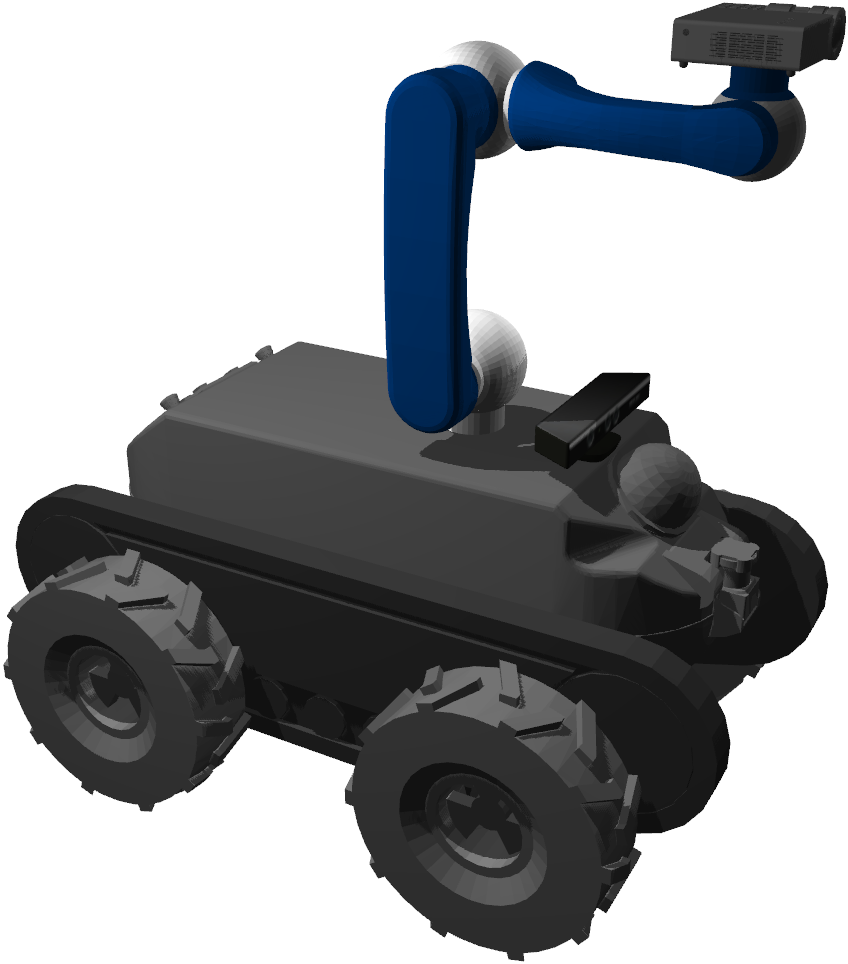
\includegraphics[width=0.7\textwidth]{localization-system-evaluation/testing-platforms/guardian-gazebo}
		\caption{Guardian Gazebo simulation}
		\label{fig:localization-system-evaluation_guardian_gazebo}
	\end{minipage}
\end{figure}


\begin{table}[H]
	\caption{\glsentryplural{lidar} hardware specifications}
	\tabulinesep = 0.8ex
	\centering
	\small
	\begin{tabu} { X[2.5,m,c] | X[m,c] X[m,c] X[m,c] X[m,c] X[m,c] }
		\rowfont{\bfseries\itshape} Laser model & Range (meters) & Field of view (degrees) & Scanning frequency (Hz) & Angular resolution (degrees) & Statistical error (millimeters) \\
		\hline
		{\small SICK NAV350} 			& [0.5..250] 	& 360 	& 8 	& 0.25 	& 15 	\\
		{\small SICK S3000} 			& [0.1..49] 	& 190 	& 8 	& 0.25 	& 150 	\\
		{\small SICK LMS200} 			& [0.1..80] 	& 180 	& 10 	& 1.0 	& 35 	\\
		{\small Hokuyo URG-04LX} 		& [0.06..4.095] & 240 	& 10 	& 0.36 	& 10 	\\
		{\small Hokuyo URG-04LX\_UG01} 	& [0.02..4] 	& 240 	& 10 	& 0.36 	& 30 	\\
	\end{tabu}
	\label{tab:localization-system-evaluation_laser-hardware-specifications}
\end{table}


\section{Testing environments}

The localization system was tested in different environments and used the Jarvis platform in a large room with a RoboCup field, the Pioneer 3-DX in a large industrial hall and the Guardian platform in a simulated indoor environment.


\subsection{Jarvis in RoboCup field}

The RoboCup field (shown in \cref{fig:localization-system-evaluation_jarvis-tests-environment} occupies half of a large room (with 20.5 meters of length and 7.7 meters of depth). It has two doors, several small windows and two large glass openings into the hallway. Several tests were performed with the robot at speeds ranging from 5 cm/s to 50 cm/s in this environment and up to 2 m/s using the Stage simulator\footnote{\url{http://rtv.github.io/Stage/}}). These tests were performed with two different movement paths. The first is a simple rounded path (shown in \cref{subsec:appendix-a_jarvis-robot-tests_rounded-path-using-the-jarvis-robot-at-5-cm-s,subsec:appendix-a_jarvis-robot-tests_rounded-path-using-the-jarvis-robot-at-30-cm-s}) that aimed to test the robot in the region of space that had better ground truth (due to its position in relation to the laser reflectors). The second path was more complex and contained several sub paths with different velocities and shapes (shown from \crefrange{subsec:appendix-a_jarvis-robot-tests_complex-path-using-the-jarvis-robot-at-5-cm-s}{subsec:appendix-a_jarvis-robot-tests_complex-path-using-the-jarvis-robot-at-50-30-50-10-cm-s-without-laser-spherical-linear-interpolation}). It was intended to evaluate the localization system with typical movements that mobile manipulators require, such as moving forward and backwards with or without angular velocity and stopping at the desired destination.


\begin{figure}[H]
	\centering
	\begin{subfigure}[h]{.497\textwidth}
		\centering
		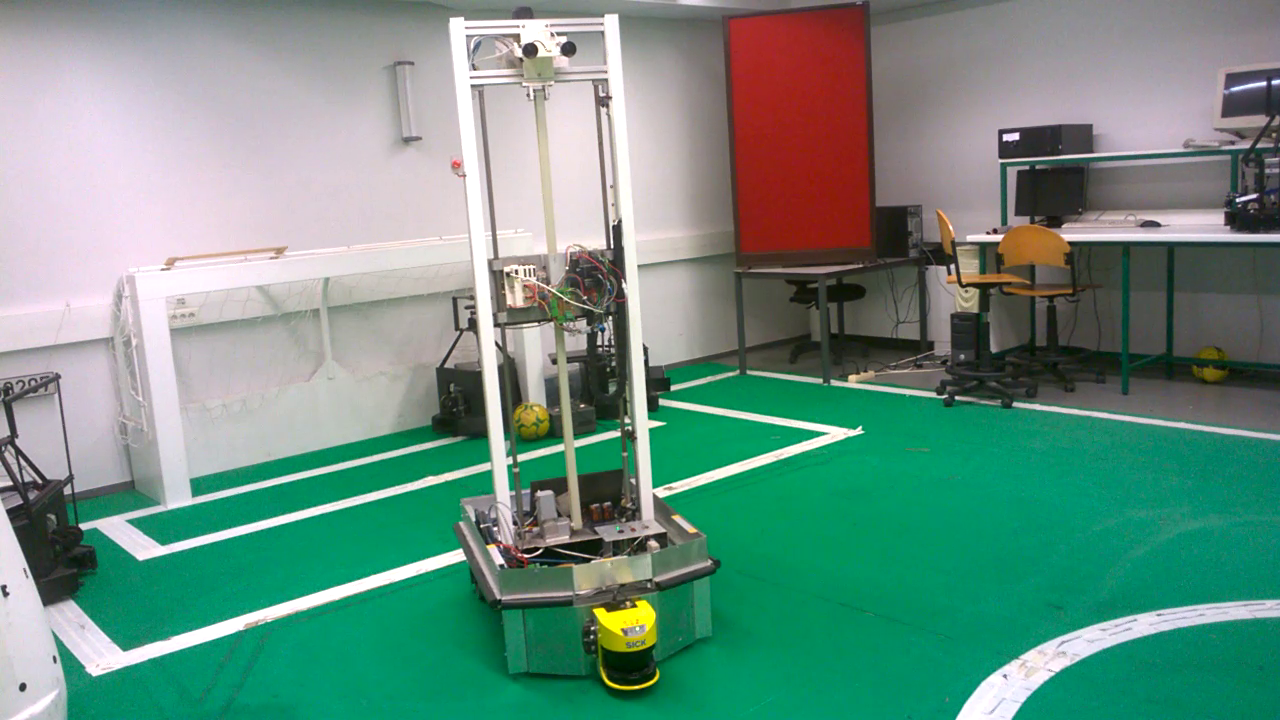
\includegraphics[width=\textwidth]{localization-system-evaluation/testing-environments/jarvis-environment-front-left}
	\end{subfigure}
	\begin{subfigure}[h]{.497\textwidth}
		\centering
		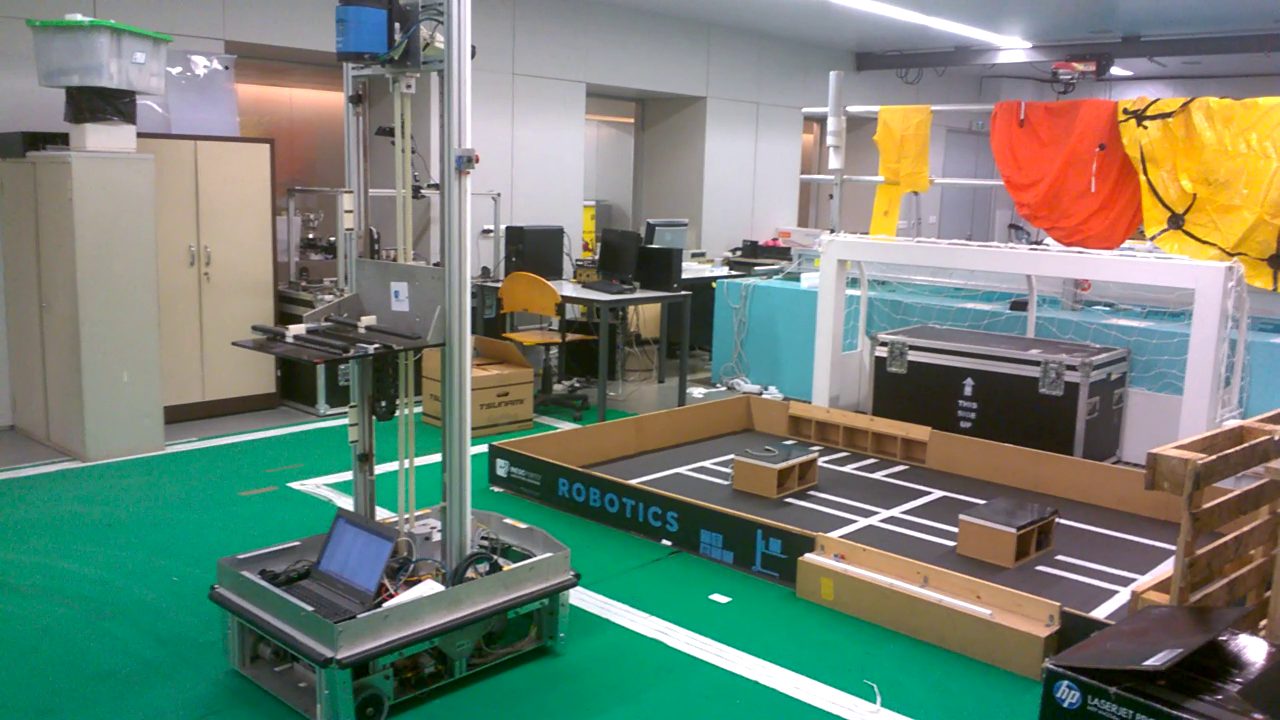
\includegraphics[width=\textwidth]{localization-system-evaluation/testing-environments/jarvis-environment-front-right}
	\end{subfigure}
	\caption{Jarvis testing environment}
	\label{fig:localization-system-evaluation_jarvis-tests-environment}
\end{figure}


\subsection{Guardian in structured environment}

The structured environment simulated in Gazebo is a large room with 12.4 meters of length and 8.4 meters of depth. It has 4 doors, several small windows and the walls have small ledges at regular intervals (as can be seen from \crefrange{fig:localization-system-evaluation_guardian-tests-environment}{fig:localization-system-evaluation_guardian-tests-environment-interactive}).

Given that the Guardian mobile manipulator is expected to work on the walls of this environment, several tests were devised with a path following the lower and right wall of the environment (shown from \crefrange{subsec:appendix-a_guardian-simulator-tests_wall-following-path-using-the-simulated-guardian-robot-at-30-cm-s-in-static-environment}{subsec:appendix-a_guardian-simulator-tests_wall-following-path-using-the-simulated-guardian-robot-at-30-cm-s-in-dynamic-cluttered-environment}). The first test was done in a static environment clear of unknown objects and was meant to evaluate the best precision that the localization system could achieve. The second test was done in a cluttered environment and was designed to test the robustness of the localization system against static unknown objects, that were placed in the middle of the environment and close to the walls (to block sensor data from reaching known positions and analyze the robustness of matching unknown points that are close to known areas). The last test added a moving car to the scene and aimed to assess the impact of dynamic objects on the point cloud registration algorithms.


\begin{figure}[H]
	\centering
	\begin{subfigure}[h]{.497\textwidth}
		\centering
		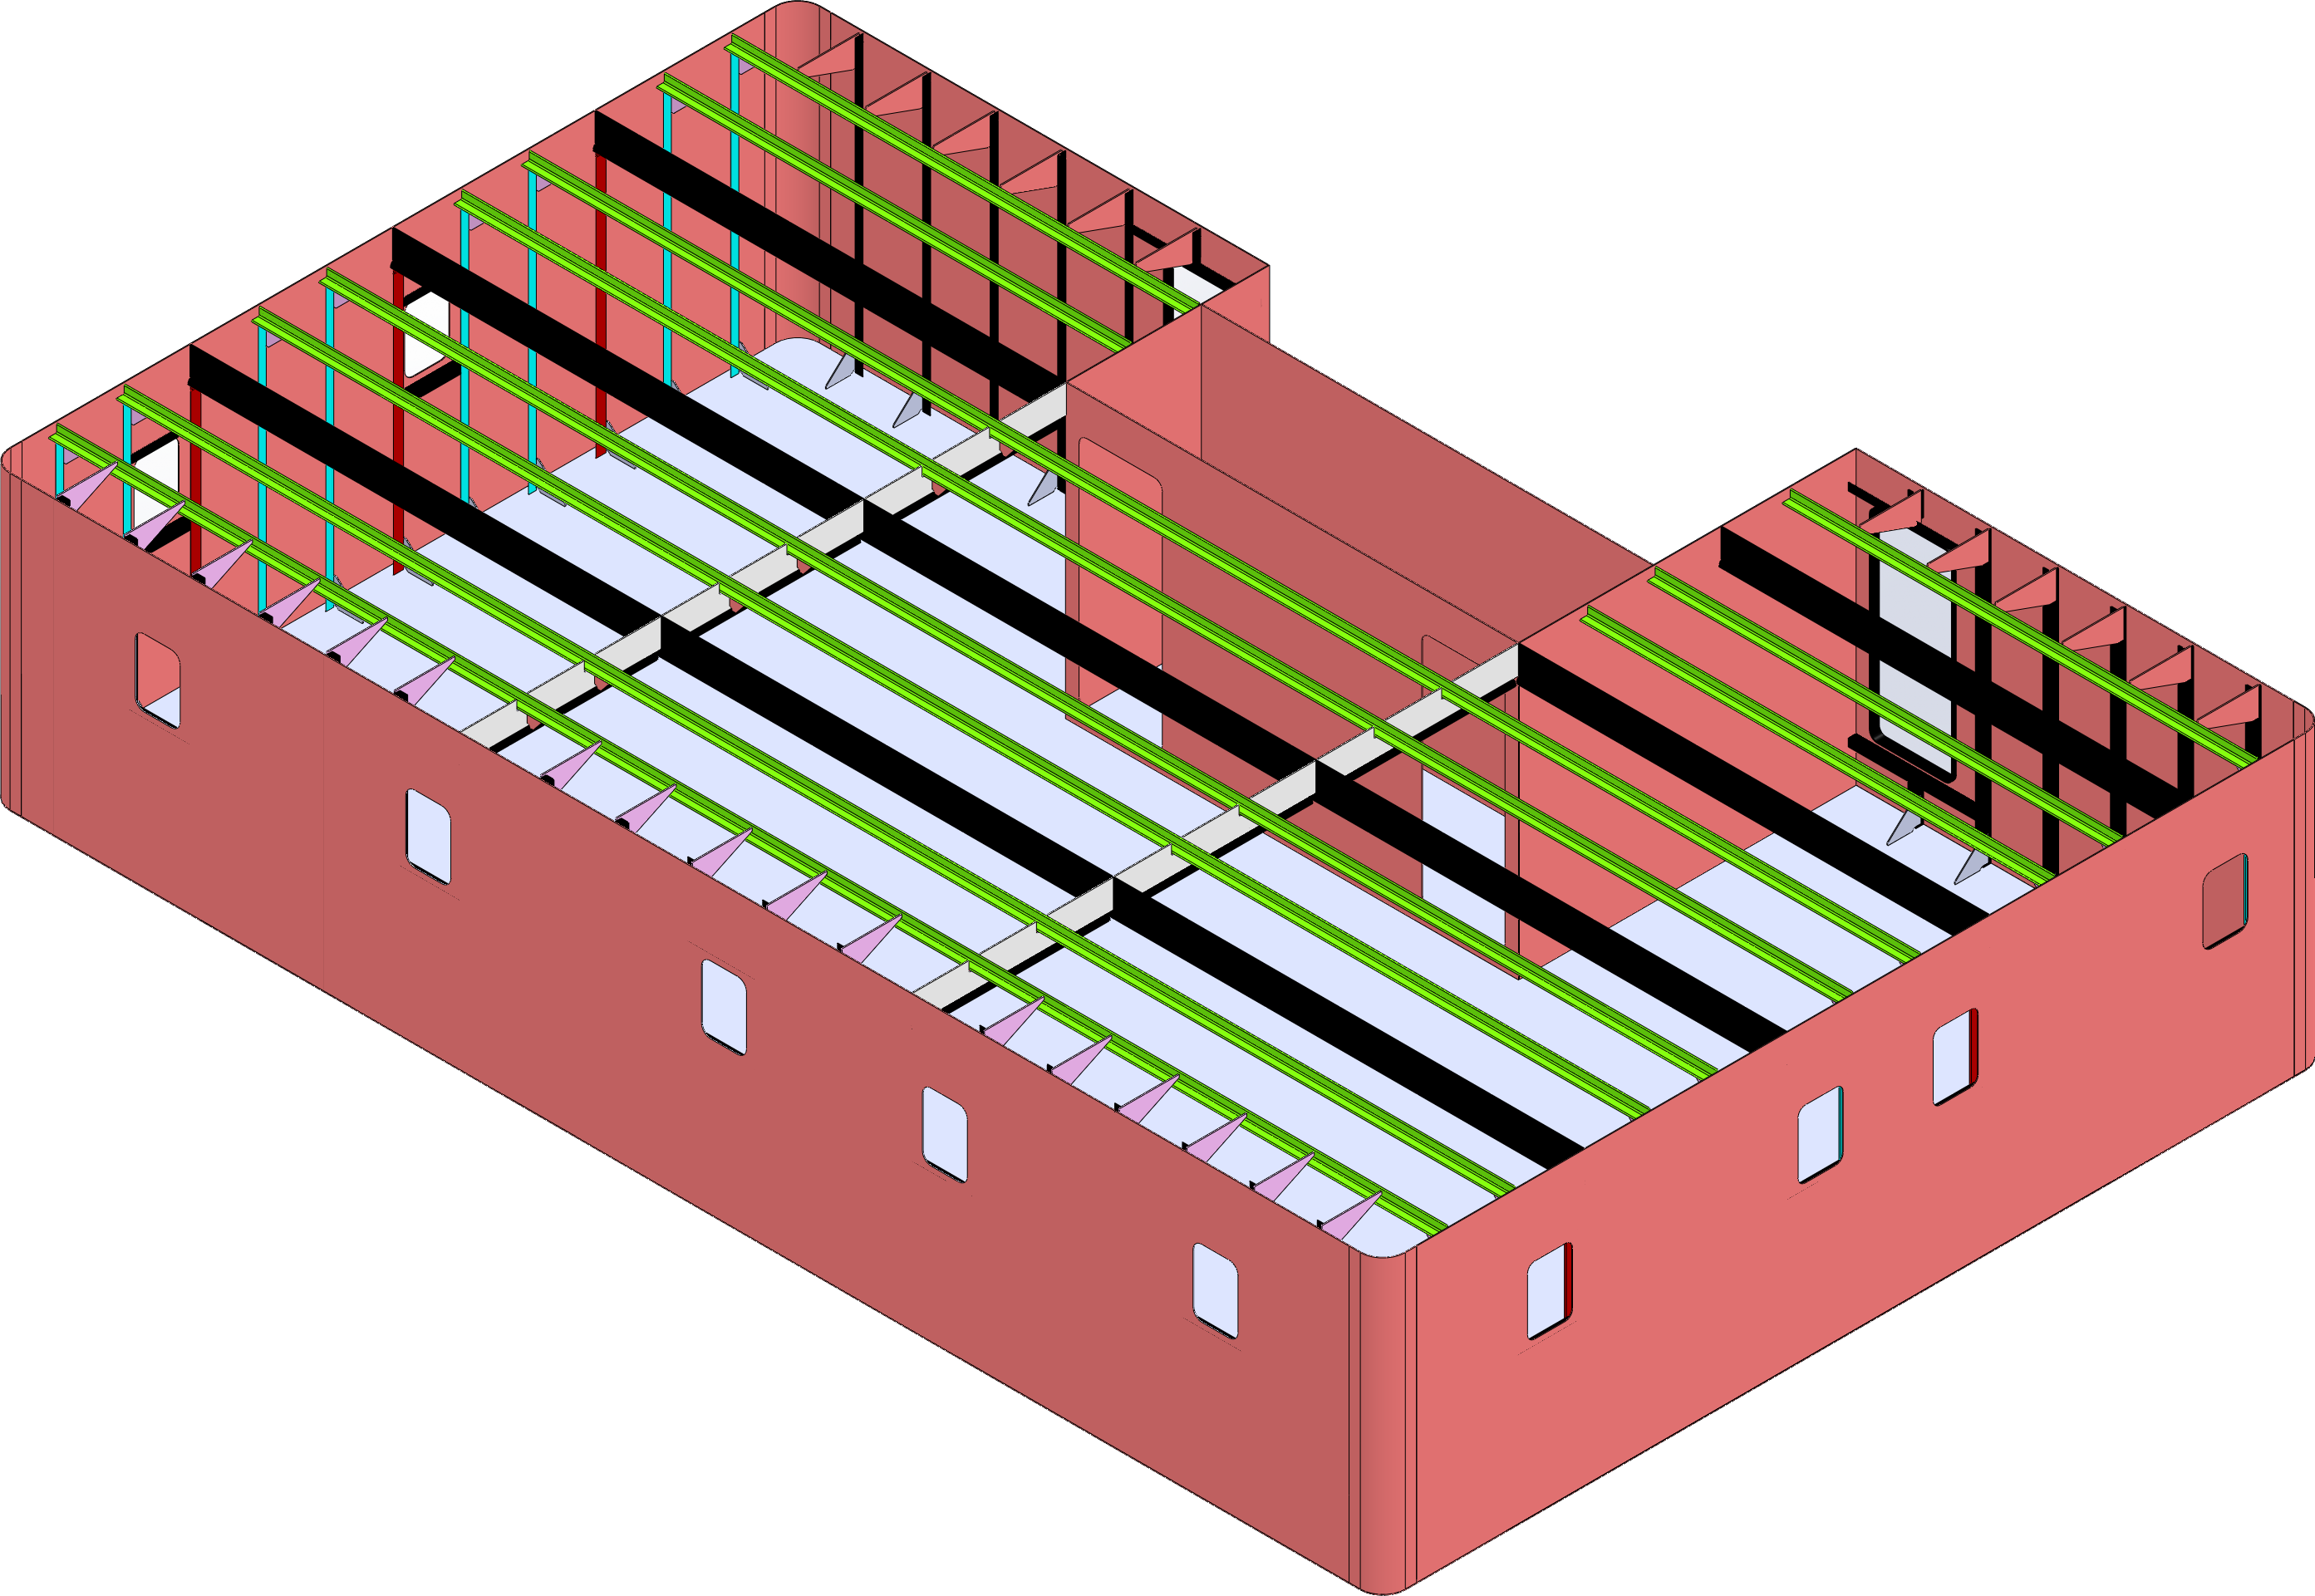
\includegraphics[width=\textwidth]{localization-system-evaluation/testing-environments/guardian-environment-corner}
	\end{subfigure}
	\begin{subfigure}[h]{.497\textwidth}
		\centering
		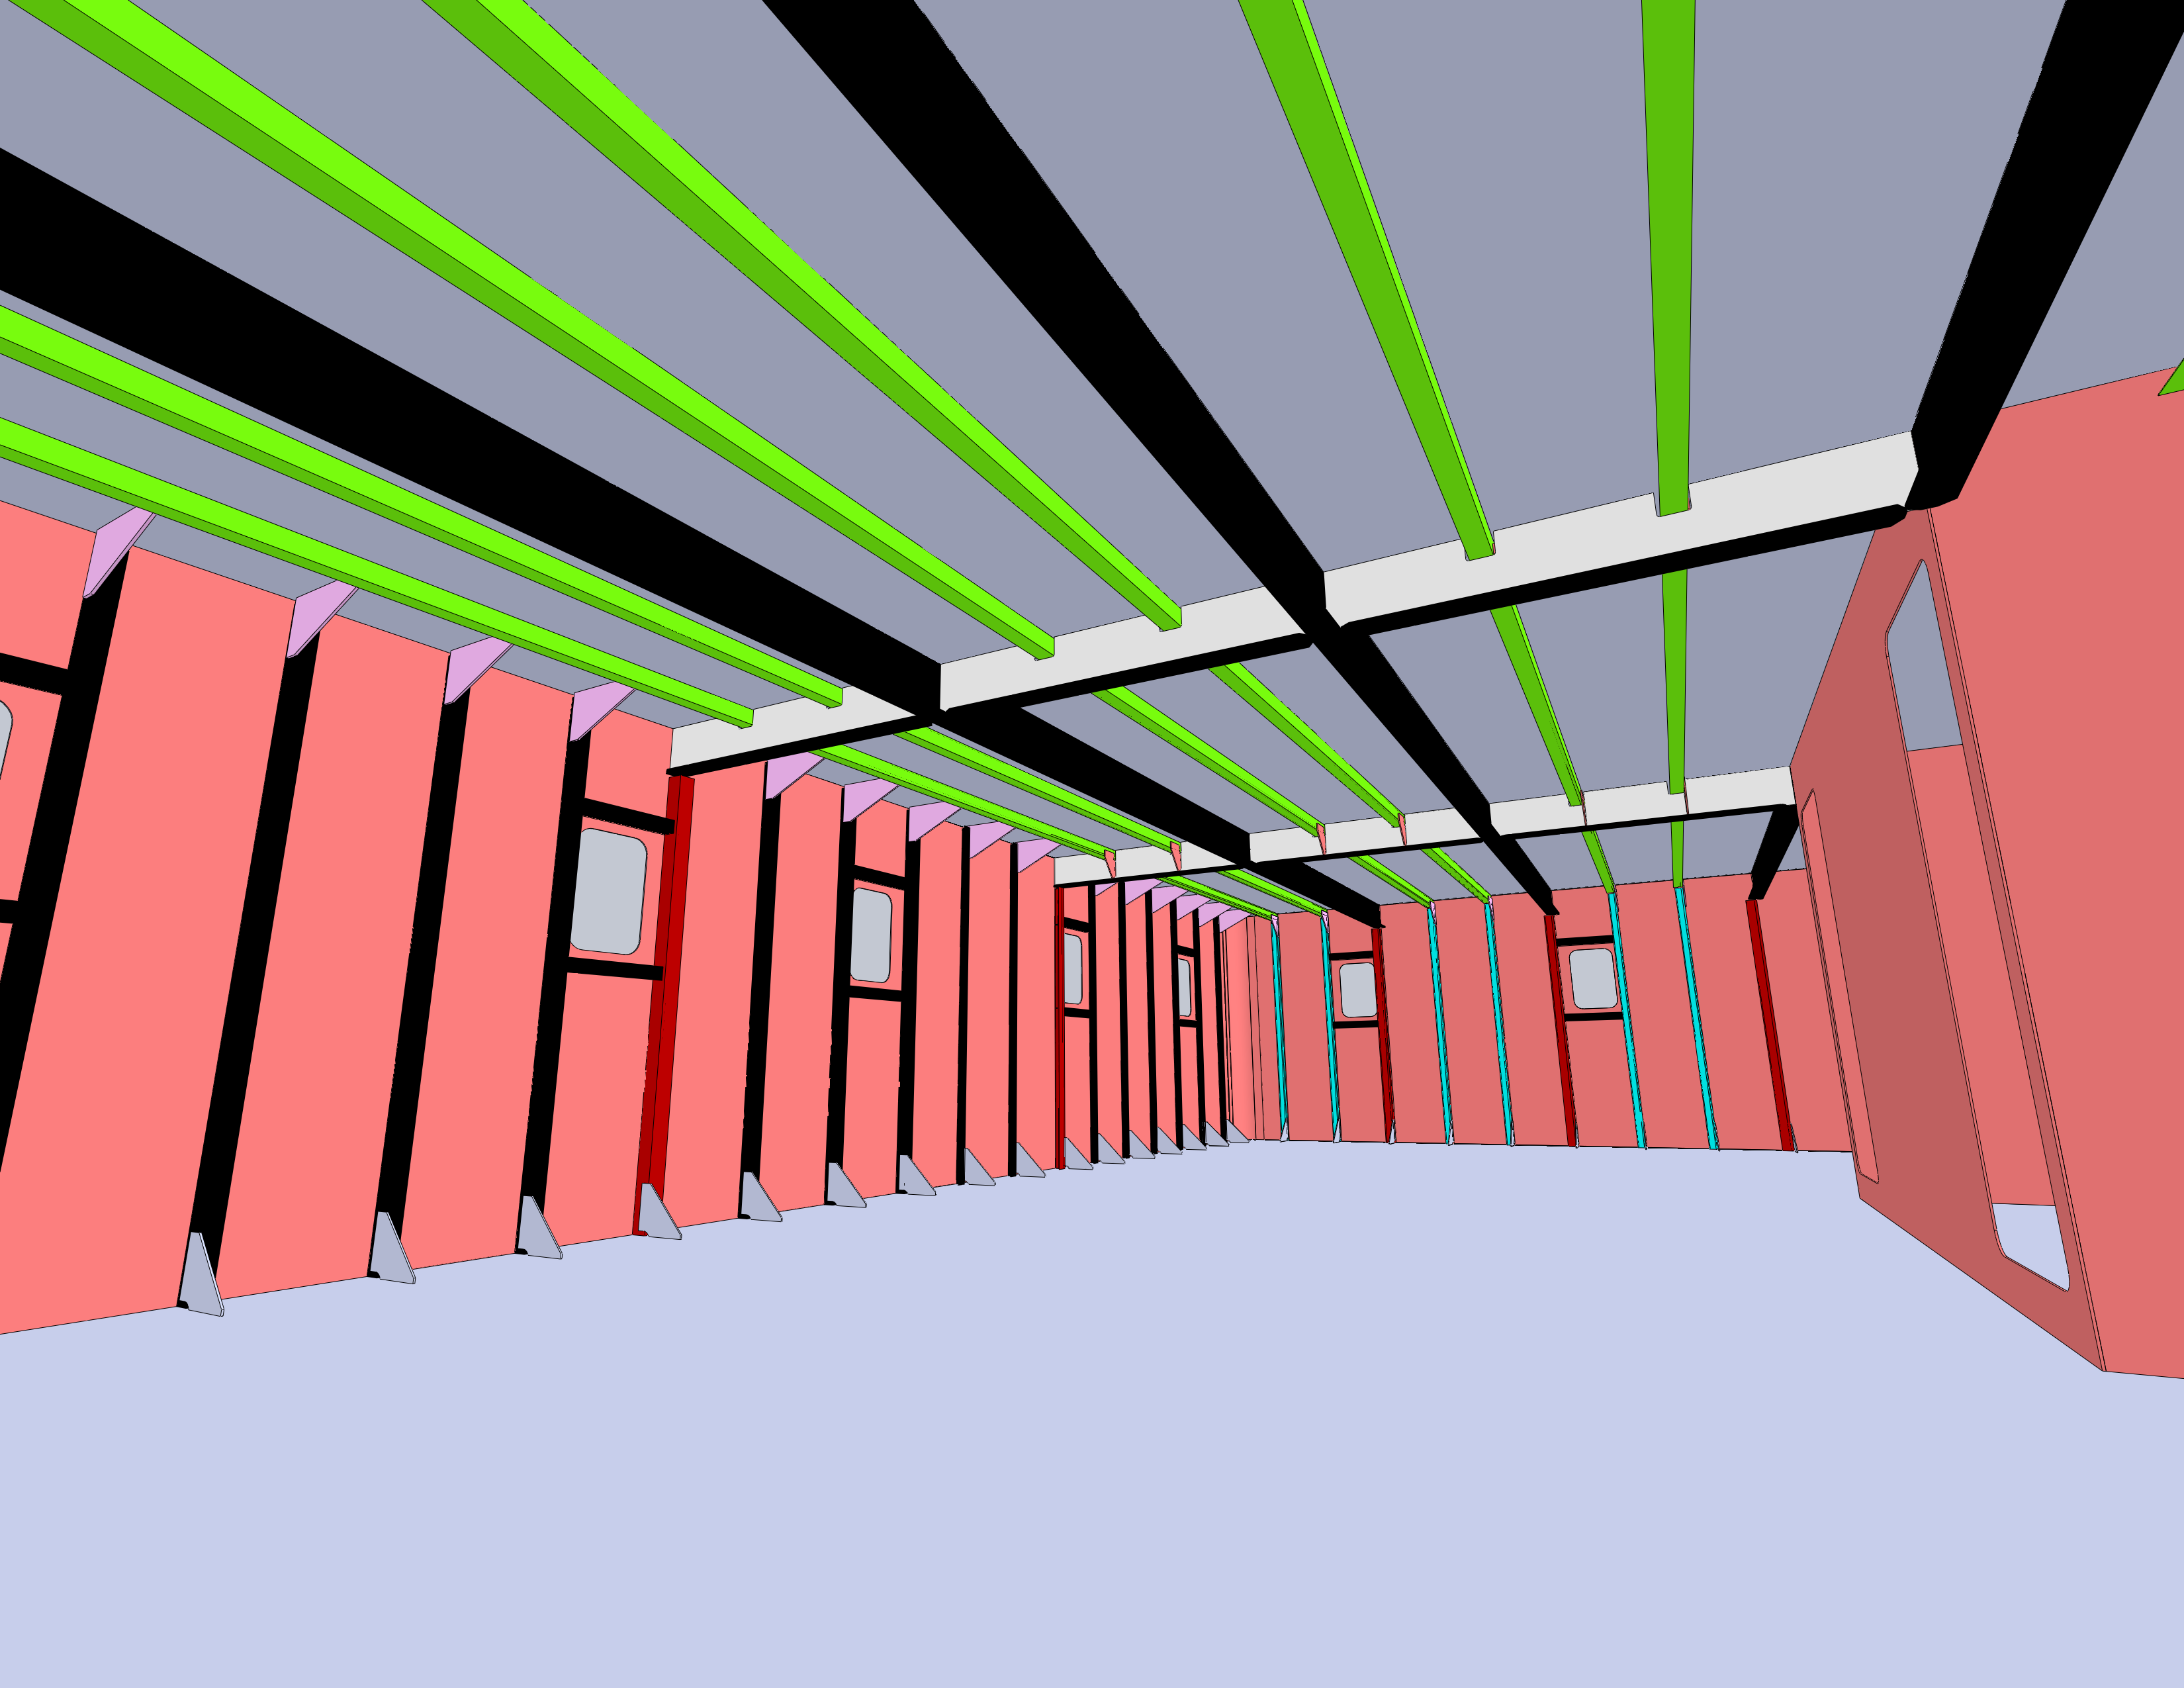
\includegraphics[width=\textwidth]{localization-system-evaluation/testing-environments/guardian-environment-inside}
	\end{subfigure}
	\caption{Guardian testing environment}
	\label{fig:localization-system-evaluation_guardian-tests-environment}
\end{figure}

\begin{figure}[H]
	\centering
	\begin{subfigure}[h]{.497\textwidth}
		\centering
		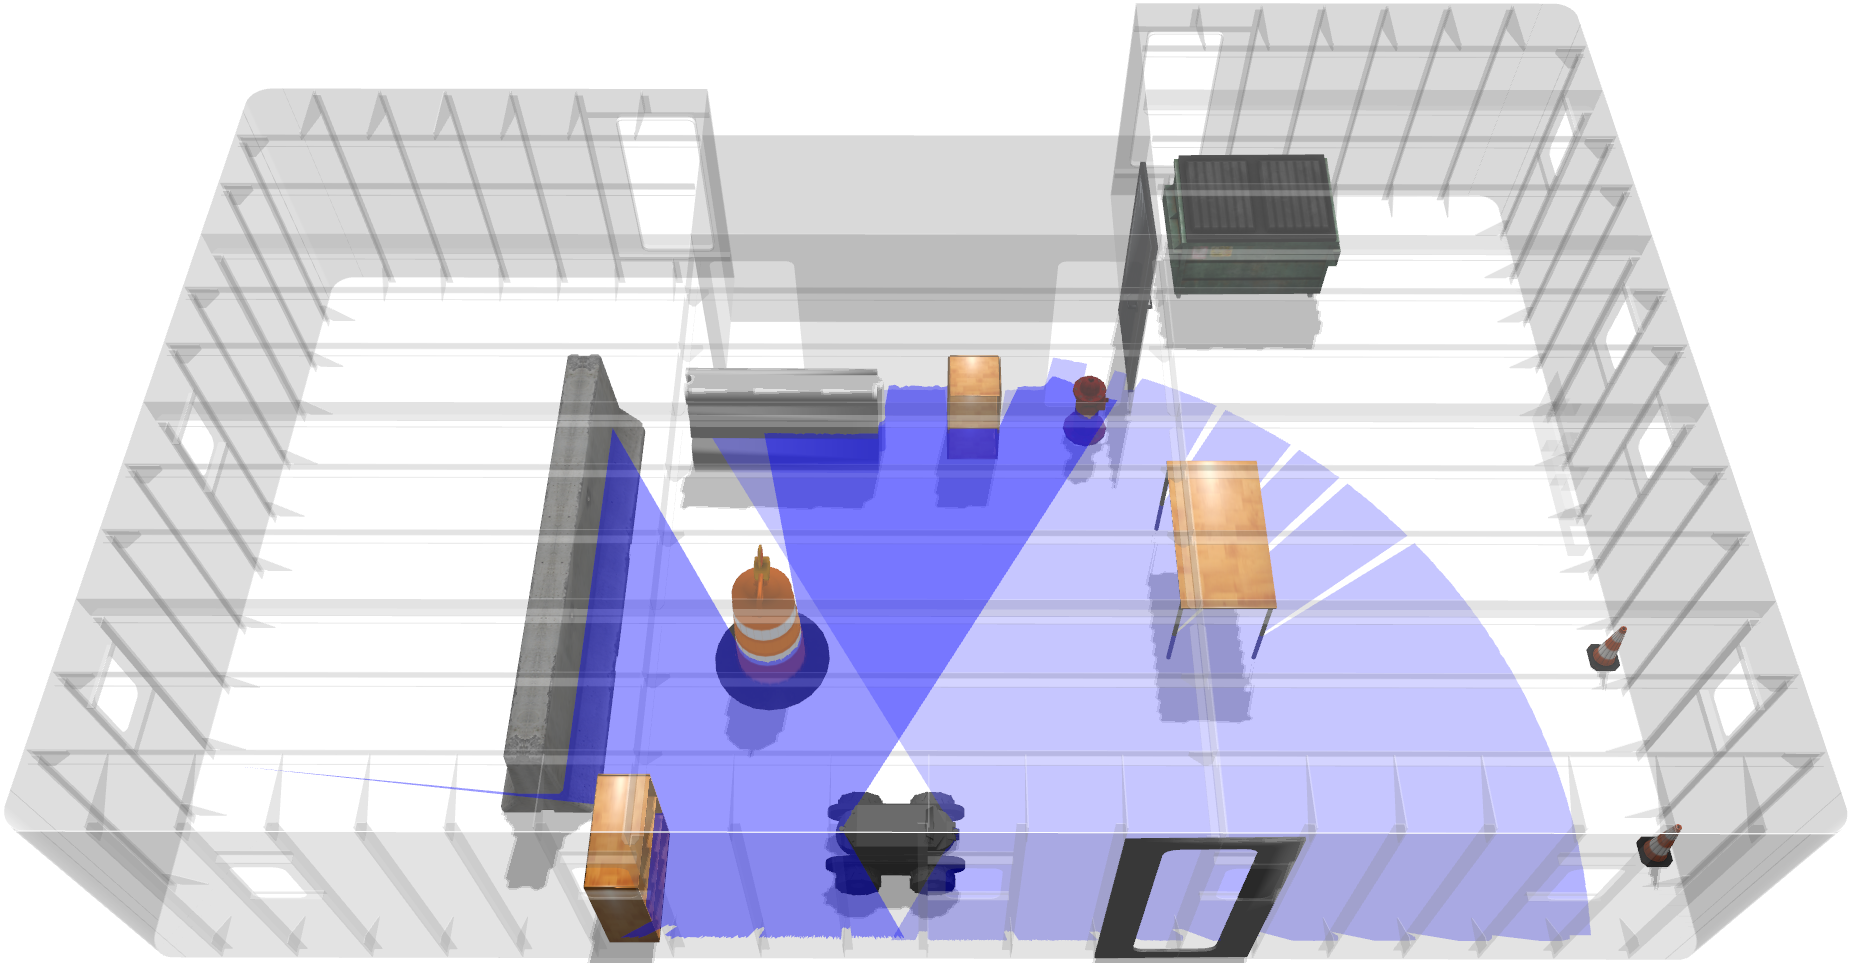
\includegraphics[width=\textwidth]{localization-system-evaluation/testing-environments/guardian-environment-cluttered}
	\end{subfigure}
	\begin{subfigure}[h]{.497\textwidth}
		\centering
		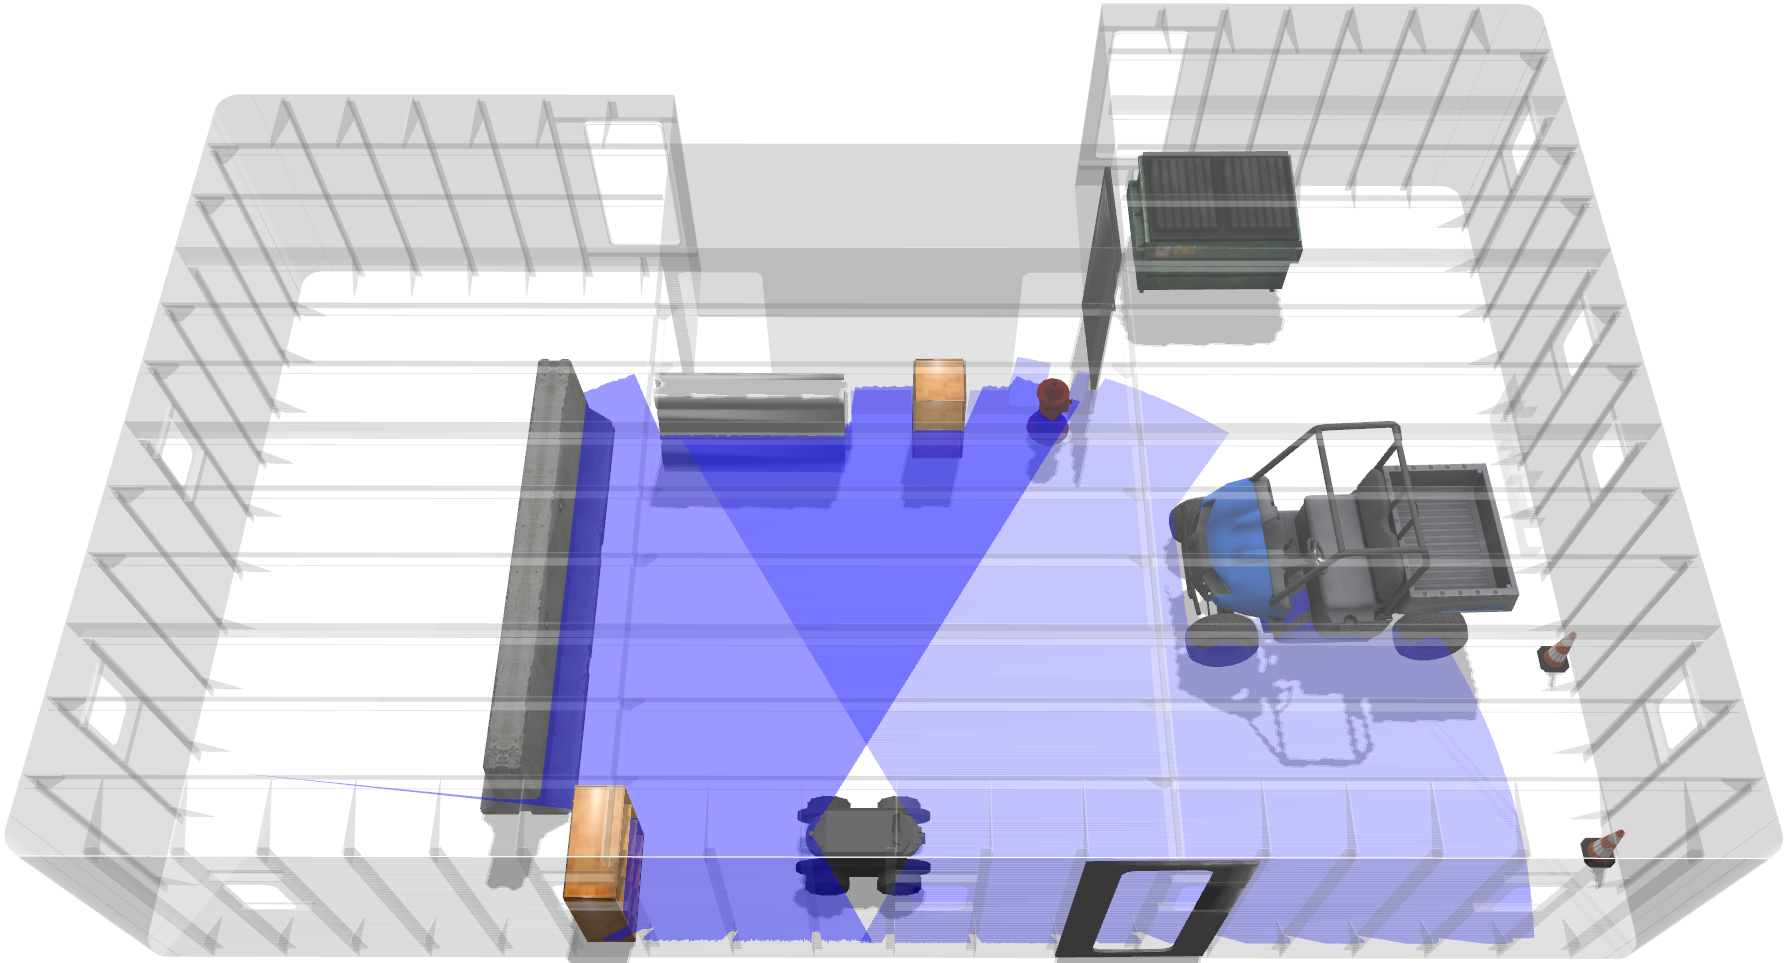
\includegraphics[width=\textwidth]{localization-system-evaluation/testing-environments/guardian-environment-cluttered_dynamic}
	\end{subfigure}
	\caption{Guardian cluttered (left) and dynamic (right) testing environment}
	\label{fig:localization-system-evaluation_guardian-tests-environment-cluttered}
\end{figure}

\begin{figure}[H]
	\centering
	\includemedia[
		label=guardian-environment,
		3Dviews=figures/localization-system-evaluation/testing-environments/guardian-environment.vws,
		width=\linewidth,
		height=0.6\linewidth,
		activate=pageopen,3Dtoolbar,3Dmenu
	]{}{figures/localization-system-evaluation/testing-environments/guardian-environment.u3d}
	\caption{Interactive \glsentrytext{cad} of Guardian testing environment (.u3d file)}
	\label{fig:localization-system-evaluation_guardian-tests-environment-interactive}
\end{figure}



\subsection{Pioneer in industrial hall}

The industrial hall is a large room with several tables and objects spread around. 4 tests were performed with the Pioneer in this environment. The first was a 360º path with few objects in the middle of the room, while the remaining 3 were done with a lot of large objects, that significantly reduced the field of view of the robot laser (as can be seen in \cref{fig:localization-system-evaluation_industrial-hall}).

\begin{figure}[H]
	\centering
	\begin{subfigure}[h]{.497\textwidth}
		\centering
		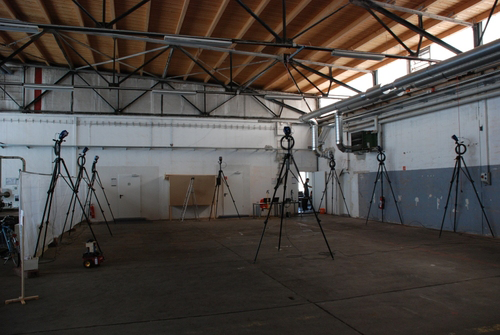
\includegraphics[width=0.95\textwidth]{localization-system-evaluation/testing-environments/industrial-hall-1}
	\end{subfigure}
	\begin{subfigure}[h]{.497\textwidth}
		\centering
		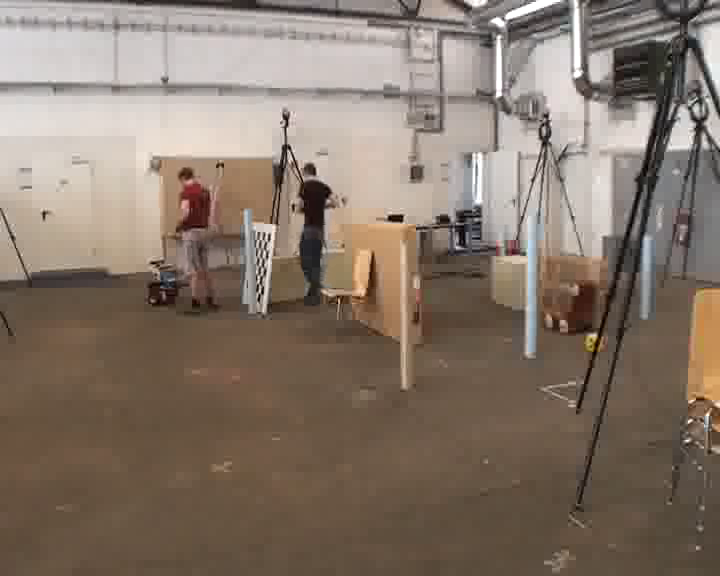
\includegraphics[width=0.8\textwidth]{localization-system-evaluation/testing-environments/industrial-hall-2}
	\end{subfigure}
	\caption{Industrial hall with and without objects in the center \cite{Sturm2012}}
	\label{fig:localization-system-evaluation_industrial-hall}
\end{figure}



\section{3 \glsentrytext{dof} localization system tests}


\subsection{Overview}

The main results of the 3 \gls{dof} tests performed with the localization system are presented in \cref{tab:localization-system-evaluation_3-dof-results,tab:localization-system-evaluation_3-dof-results-odometry-amcl}. They summarizes each test by fitting a normal distribution for each evaluation metric. They were retrieved with a known initial pose using \gls{icp} point-to-point as tracking algorithm and \gls{icp} point-to-plane as tracking recovery method. The Jarvis and Pioneer tests had a map built using the localization system in \gls{slam} mode and were manually corrected to achieve a resolution of 10 and 25 mm respectively. The Guardian tests relied on a map built from the \gls{cad} model with resolution of 2 mm. A voxel grid of 50 mm was applied to the assembled laser scans in order to reduce the impact of sensor measurement noise and also control the level of detaild of the point clouds. The initial pose estimation subsystem used \gls{sift} for keypoint selection, \gls{fpfh} for keypoint description and the feature matching algorithm described in \cref{subsec:localization-system_feature-registration} to estimate the initial position and orientation of the robot (\cref{fig:localization-system-evaluation_ship-interior-initial-pose-estimation-sift-fpfh-ransac-gicp} shows the accepted initial poses when the robot was in the lower right corner of the Guardian test environment).

The next sections will provide an overview analysis of the main 3 \gls{dof} results achieved with the proposed localization system (available in \cref{app:appendix-a}). It will start by explaining how laser spherical interpolation can mitigate point cloud deformation. Later on it will analyze the point cloud preprocessing stage and why it should be carefully tuned to the sensors and ambient geometry. Next it will present the \gls{slam} problem and why it is necessary to have accurate maps in order to achieve precise localization. Finally it will be presented a detailed analysis of 3 of the most representative tests, in which the results achieved by the proposed localization system will be compared with the ground truth, odometry and \gls{amcl}.

\clearpage

\begin{sidewaystable}
	\caption{3 \glsentrytext{dof} localization system results - (*) Most relevant experiments}
	\tabulinesep = 1.2ex
	\setlength{\tabcolsep}{0.2em}
	\centering
	\tiny
	\begin{tabu} to \textwidth { X[m,c] X[m,c] X[m,c] X[m,c] X[1.7m,c] X[m,c] X[m,c] X[0.01m,c] X[m,c] X[m,c] X[0.01m,c] X[m,c] X[m,c] X[0.01m,c] X[m,c] X[m,c] X[0.01m,c] X[m,c] X[m,c] }
		\hline
		\multicolumn{7}{c}{Test conditions} && \multicolumn{2}{c}{Translation error (millimeters)} && \multicolumn{2}{c}{Rotation error (degrees)} && \multicolumn{2}{c}{Outliers percentage [0..100]} && \multicolumn{2}{c}{Global computation time (milliseconds)} \\
		\cline{1-7} \cline{9-10} \cline{12-13} \cline{15-16} \cline{18-19}
		Section 	& Platform 																& Ambient 													& Path shape 											& Path velocities 		& Map cell resolution 	& Nº scans / Nº lasers 	&& Mean   & Standard deviation 	&& Mean  & Standard deviation 	&& Mean  & Standard deviation 	&& Mean   & Standard deviation \\ \hline
		A.1.1		& \multirow{4}{0.05\textwidth}{\centering Jarvis robot} 				& \multirow{2}{0.05\textwidth}{\centering Cluttered} 		& \multirow{2}{0.05\textwidth}{\centering Rounded} 		& 5 cm/s 				& 10 mm					& 1-4/1 				&& 3.384  & 1.900 				&& 0.549 & 0.087 				&& 15.75 & 3.84 				&& 12.052 & 12.232	\\
		A.1.2		&																		&															&														& 30 cm/s				& 10 mm					& 1-4/1					&& 12.250 & 8.901				&& 0.535 & 0.414				&& 16.08 & 3.80					&& 21.295 &	8.352	\\ \tabucline[0.5pt on 3pt off 2pt]{3-4}
		A.1.3		&																		& \multirow{2}{0.05\textwidth}{\centering Cluttered dynamic}& \multirow{2}{0.05\textwidth}{\centering Complex} 		& 5 cm/s 				& 10 mm					& 1-4/1			 		&& 4.280  & 2.264 				&& 0.441 & 0.070 				&& 24.35 & 5.17 				&& 11.776 & 12.265	\\
		A.1.4 (*)	&																		&															&														& {50-30-50-10 cm/s}	& 10 mm					& 1-4/1					&& 6.422  &	3.992				&& 0.397 & 0.099				&& 23.84 & 5.59					&& 13.376 &	13.316	\\ \tabucline[0.5pt on 3pt off 2pt]{1-4}
		A.2.1		& \multirow{4}{0.05\textwidth}{\centering Pioneer robot}				& \multirow{4}{0.05\textwidth}{\centering Cluttered dynamic}& 360º													& 23 cm/s				& 25 mm					& 1/1					&& 20.105 & 10.814				&& 5.704 & 0.662				&& 11.71 & 3.37					&& 5.046  & 2.106	\\
		A.2.2		&																		&															& SLAM 1												& 26 cm/s				& 25 mm					& 1/1					&& 22.434 & 12.052				&& 5.429 & 0.676				&& 4.31  & 3.84					&& 4.569  & 2.530	\\
		A.2.3		&																		&															& SLAM 2												& 19 cm/s				& 25 mm					& 1/1					&& 19.391 & 12.568				&& 5.518 & 0.818				&& 5.09  & 4.11					&& 4.650  & 2.180	\\
		A.2.4 (*)	&																		&															& SLAM 3												& 16 cm/s				& 25 mm					& 1/1					&& 17.480 & 8.895				&& 5.455 & 0.732				&& 4.15  & 4.26					&& 4.388  & 2.526	\\ \tabucline[0.5pt on 3pt off 2pt]{1-4}
					& \multirow{6}{0.05\textwidth}{\centering Jarvis simulator (Stage)} 	& \multirow{6}{0.05\textwidth}{\centering Cluttered} 		& \multirow{3}{0.05\textwidth}{\centering Rounded} 		& 5 cm/s 				& 10 mm					& 2/1					&& 2.817  & 1.551 				&& 0.038 & 0.026 				&& 16.11 & 0.93 				&& 12.600 & 12.459 	\\
					&																		&  															&  														& 50 cm/s 				& 10 mm					& 2/1					&& 4.479  & 3.769 				&& 0.106 & 0.137 				&& 15.82 & 1.14 				&& 24.500 & 13.592 	\\
					&																		&  															&  														& 100 cm/s 				& 10 mm					& 1/1 					&& 4.710  & 2.788 				&& 0.135 & 0.134 				&& 16.13 & 0.92 				&& 16.432 & 12.291 	\\ \tabucline[0.5pt on 3pt off 2pt]{4-4}
					&																		&  															& \multirow{3}{0.05\textwidth}{\centering Complex} 		& 5 cm/s 				& 10 mm					& 2/1 					&& 2.476  & 1.370 				&& 0.017 & 0.017 				&& 17.00 & 0.92 				&& 10.374 & 12.138 	\\
					&																		&  															&  														& 50-30-50-20 cm/s 		& 10 mm					& 2/1					&& 3.557  & 1.800 				&& 0.033 & 0.040 				&& 17.61 & 1.33 				&& 14.863 & 15.898 	\\
					&																		&  															&  														& 200-30-200-30 cm/s 	& 10 mm					& 2/1					&& 4.199  & 2.596 				&& 0.048 & 0.110 				&& 17.84 & 1.23 				&& 13.150 & 14.351 	\\ \tabucline[0.5pt on 3pt off 2pt]{1-4}
					& \multirow{6}{0.05\textwidth}{\centering Guardian simulator (Gazebo)} 	& \multirow{2}{0.05\textwidth}{\centering Static} 			& \multirow{6}{0.05\textwidth}{\centering Wall follower}& 5 cm/s 				& 2 mm					& 2/2 					&& 2.642  & 0.463 				&& 0.016 & 0.023 				&& 0.0   & 0.0  				&& 5.723  & 1.868 	\\
		A.3.1		&																		&  															&  														& 30 cm/s 				& 2 mm					& 2-4/2					&& 4.654  & 3.893 				&& 0.044 & 0.070 				&& 0.0   & 0.0  				&& 7.784  & 3.178 	\\ \tabucline[0.5pt on 3pt off 2pt]{3-3}
					&																		& \multirow{2}{0.05\textwidth}{\centering Cluttered} 		&  														& 5 cm/s 				& 2 mm					& 2/2					&& 2.912  & 0.856 				&& 0.020 & 0.026 				&& 25.05 & 13.30 				&& 11.889 & 9.084 	\\
		A.3.2		&																		&  															& 														& 30 cm/s 				& 2 mm					& 2-4/2					&& 6.092  & 3.834 				&& 0.096 & 0.085 				&& 25.65 & 11.02 				&& 23.925 & 27.959 	\\ \tabucline[0.5pt on 3pt off 2pt]{3-3}
					&																		& \multirow{2}{0.05\textwidth}{\centering Cluttered dynamic}&  														& 5 cm/s 				& 2 mm					& 2/2					&& 4.593  & 3.802 				&& 0.069 & 0.072 				&& 33.33 & 9.88  				&& 22.217 & 32.408 	\\
		A.3.3 (*)	&																		&  															&  														& 30 cm/s 				& 2 mm					& 2/2					&& 5.897  & 4.452 				&& 0.095 & 0.104 				&& 27.28 & 13.04 				&& 24.409 & 33.459 	\\
		\hline
	\end{tabu}
	\label{tab:localization-system-evaluation_3-dof-results}
\end{sidewaystable}


\begin{sidewaystable}
	\caption{3 \glsentrytext{dof} odometry and \glsentrytext{amcl} results - (*) Most relevant experiments}
	\tabulinesep = 1.2ex
	\setlength{\tabcolsep}{0.2em}
	\centering
	\tiny
	\begin{tabu} to \textwidth { X[m,c] X[m,c] X[m,c] X[m,c] X[1.7m,c] X[m,c] X[0.01m,c] X[m,c] X[m,c] X[0.01m,c] X[m,c] X[m,c] X[0.01m,c] X[m,c] X[m,c] X[0.01m,c] X[m,c] X[m,c] }
		\hline
		\multicolumn{6}{c}{Test conditions} && \multicolumn{2}{c}{Odometry translation error (millimeters)} && \multicolumn{2}{c}{Odometry rotation error (degrees)} && \multicolumn{2}{c}{\glsentrytext{amcl} translation error (millimeters)} && \multicolumn{2}{c}{\glsentrytext{amcl} rotation error (degrees)} \\
		\cline{1-6} \cline{8-9} \cline{11-12} \cline{14-15} \cline{17-18}
		Section 	& Platform 																& Ambient 													& Path shape 											& Path velocities 		& Map cell resolution 	&& Mean   	& Standard deviation 	&& Mean  	& Standard deviation 	&& Mean  	& Standard deviation 	&& Mean   & Standard deviation \\ \hline
		A.1.1 		& \multirow{4}{0.05\textwidth}{\centering Jarvis robot} 				& \multirow{2}{0.05\textwidth}{\centering Cluttered} 		& \multirow{2}{0.05\textwidth}{\centering Rounded} 		& 5 cm/s 				& 10 mm					&& 25.353 	& 10.075 				&& 0.352 	& 0.206 				&& 51.417	& 20.829 				&& 0.442  & 0.174	\\
		A.1.2		&																		&															&														& 30 cm/s				& 10 mm					&& 103.676	& 50.992				&& 2.173 	& 1.916					&& 81.368	& 36.548				&& 1.388  &	1.085	\\ \tabucline[0.5pt on 3pt off 2pt]{3-4}
		A.1.3		&																		& \multirow{2}{0.05\textwidth}{\centering Cluttered dynamic}& \multirow{2}{0.05\textwidth}{\centering Complex} 		& 5 cm/s 				& 10 mm					&& 21.506 	& 11.937 				&& 0.535 	& 0.360 				&& 64.300	& 13.750 				&& 0.316  & 0.214	\\
		A.1.4 (*)	&																		&															&														& 50-30-50-10 cm/s		& 10 mm					&& 124.269	&	79.775				&& 2.723 	& 1.496					&& 84.230	& 29.134				&& 0.595  &	0.581	\\ \tabucline[0.5pt on 3pt off 2pt]{1-4}
		A.2.1		& \multirow{4}{0.05\textwidth}{\centering Pioneer robot}				& \multirow{4}{0.05\textwidth}{\centering Cluttered dynamic}& 360º													& 23 cm/s				& 25 mm					&& 482.439	& 163.657				&& 12.810	& 4.468					&& 135.442	& 66.445				&& 6.462  & 1.290	\\
		A.2.2		&																		&															& SLAM 1												& 26 cm/s				& 25 mm					&& 370.283 	& 163.734				&& 8.351 	& 2.825					&& 111.470 	& 46.783				&& 6.496  & 1.386	\\
		A.2.3		&																		&															& SLAM 2												& 19 cm/s				& 25 mm					&& 686.983 	& 361.666				&& 11.333 	& 5.423					&& 95.537  	& 47.560				&& 6.957  & 2.294	\\
		A.2.4 (*)	&																		&															& SLAM 3												& 16 cm/s				& 25 mm					&& 295.714 	& 151.793				&& 8.858 	& 3.331					&& 108.690 	& 52.341				&& 6.463  & 1.363	\\
		\hline
	\end{tabu}
	\label{tab:localization-system-evaluation_3-dof-results-odometry-amcl}
\end{sidewaystable}


\clearpage

\subsection{Laser assembly with spherical linear interpolation}

The localization system was designed to operate with point cloud sensors (such as the ones presented in \cref{sec:relevant-sofware-hardware-technologies_point-cloud-acquisition}). For the particular case of data retrieved using \glspl{lidar}, there is a very significant problem of point cloud deformation when the robot is moving or rotating at high speeds. This is due to the fact that a typical \gls{lidar} outputs laser scans at a very low rate (8-10 Hz), and as such, assuming that the robot isn't moving when capturing an entire scan will result in deformed point clouds. Given that \gls{ros} outputs laser scans (an entire slice of laser measurements from the start to the end of its field of view), and the localization system doesn't have access to individual measurements as they arrive, then one way to mitigate this deformation is by using odometry and / or \gls{imu} information to update the robot pose between the pose corrections performed by the localization system. This allows to use spherical linear interpolation when converting from the raw measurements in polar coordinates into the required Cartesian coordinates in the map frame.

As can be seen in \cref{subsec:appendix-a_jarvis-robot-tests_complex-path-using-the-jarvis-robot-at-5-cm-s-without-laser-spherical-linear-interpolation}, laser scan deformation is negligible when the robot is moving very slowly. However, when moving at higher speeds, the point cloud deformation poses a serious issue, and the usage of spherical linear interpolation is very important to mitigate it (demonstrated in \cref{subsec:appendix-a_jarvis-robot-tests_complex-path-using-the-jarvis-robot-at-50-30-50-10-cm-s-without-laser-spherical-linear-interpolation}).

In \cref{fig:localization-system-evaluation_laser-deformation-1} can be seen that the laser measurements in front of the robot were deformed outwards, causing the points to be projected outside both walls. \Cref{fig:localization-system-evaluation_laser-deformation-2} shows the same effect, which is now very noticeable since the first laser measurement isn't close to the last one. These deformations were severely diminished when the laser spherical linear interpolation was used (as can be seen in \cref{fig:localization-system-evaluation_laser-deformation-1-corrected,fig:localization-system-evaluation_laser-deformation-2-corrected,fig:appendix-a_jarvis-robot-tests_complex-path-using-the-jarvis-robot-at-50-30-50-10-cm-s-without-laser-spherical-linear-interpolation_lasers-with-interpolation,fig:appendix-a_jarvis-robot-tests_complex-path-using-the-jarvis-robot-at-50-30-50-10-cm-s-without-laser-spherical-linear-interpolation_lasers-without-interpolation} respectively.


\begin{figure}[H]
	\centering
	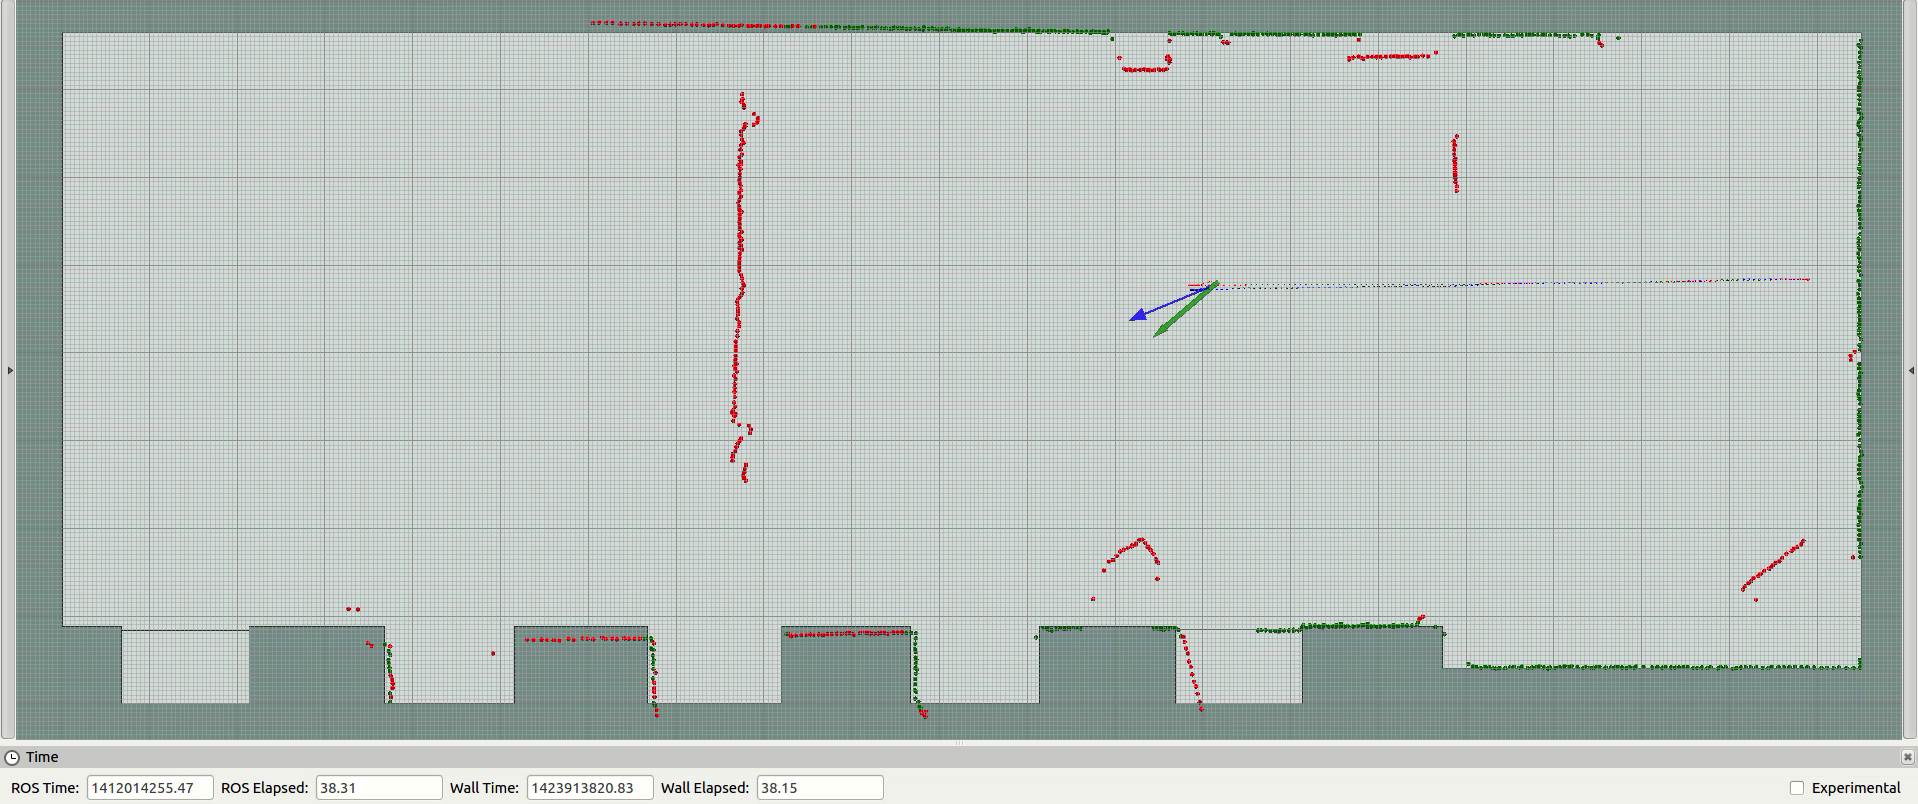
\includegraphics[width=0.97\textwidth]{localization-system-evaluation/tests-3dof/laser-spherical-interpolation/laser-deformation-1}
	\caption{Large laser deformation on opposite walls when the robot is rotating}
	\label{fig:localization-system-evaluation_laser-deformation-1}
\end{figure}

\begin{figure}[H]
	\centering
	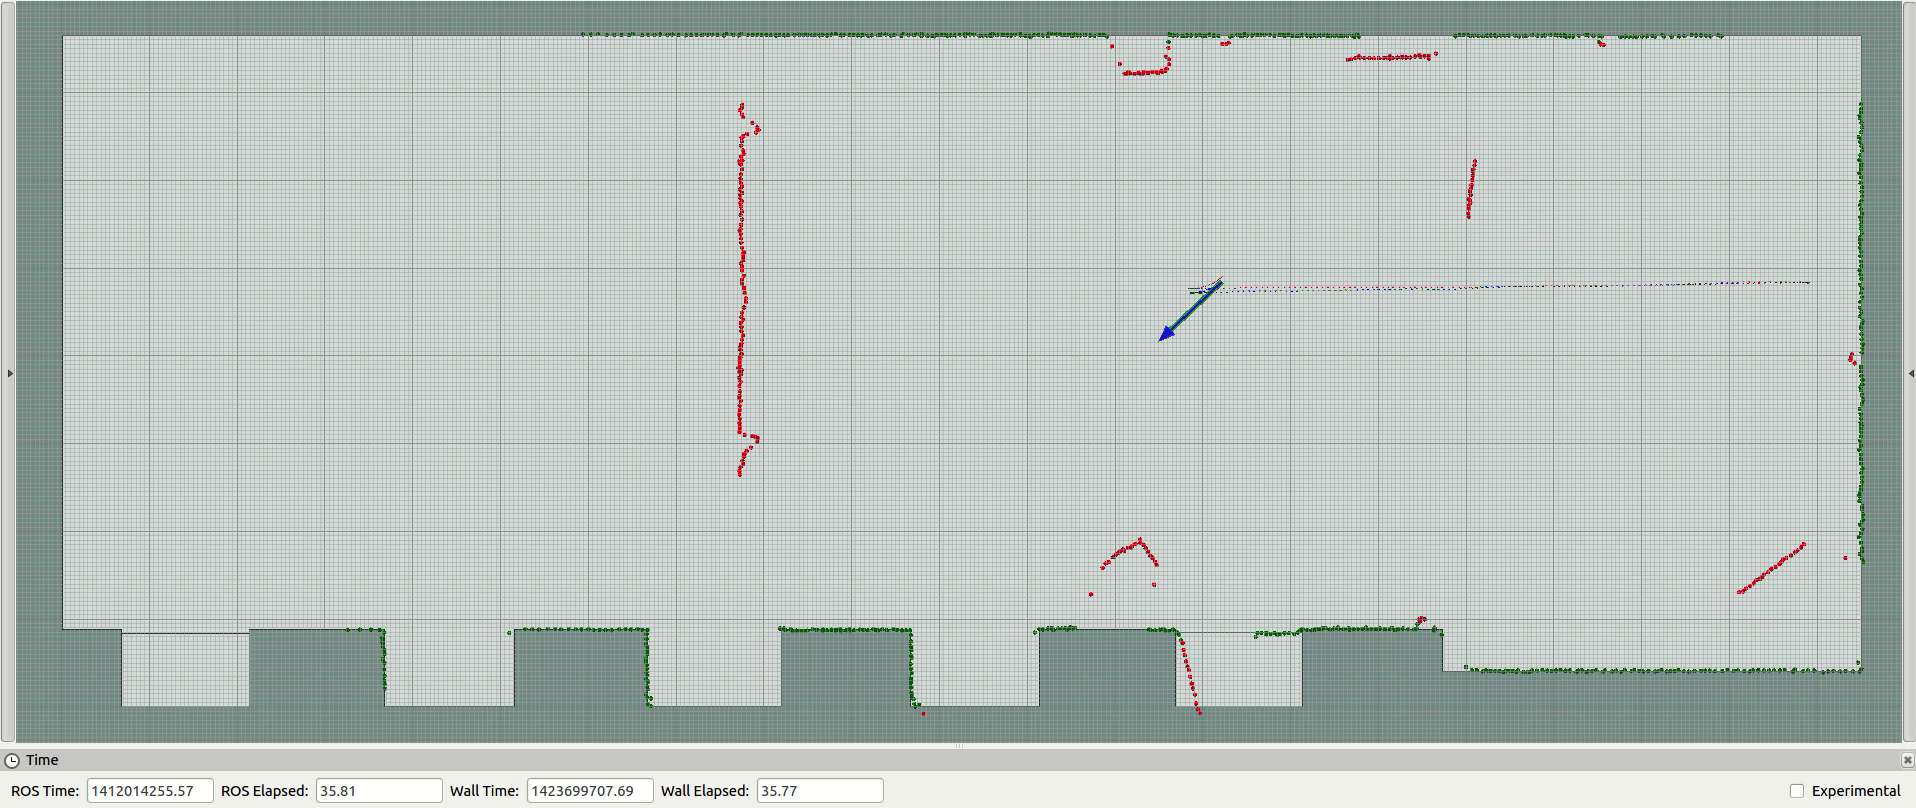
\includegraphics[width=0.97\textwidth]{localization-system-evaluation/tests-3dof/laser-spherical-interpolation/laser-deformation-1-corrected}
	\caption{Correction of the large laser deformation on opposite walls with spherical linear interpolation}
	\label{fig:localization-system-evaluation_laser-deformation-1-corrected}
\end{figure}


\begin{figure}[H]
	\centering
	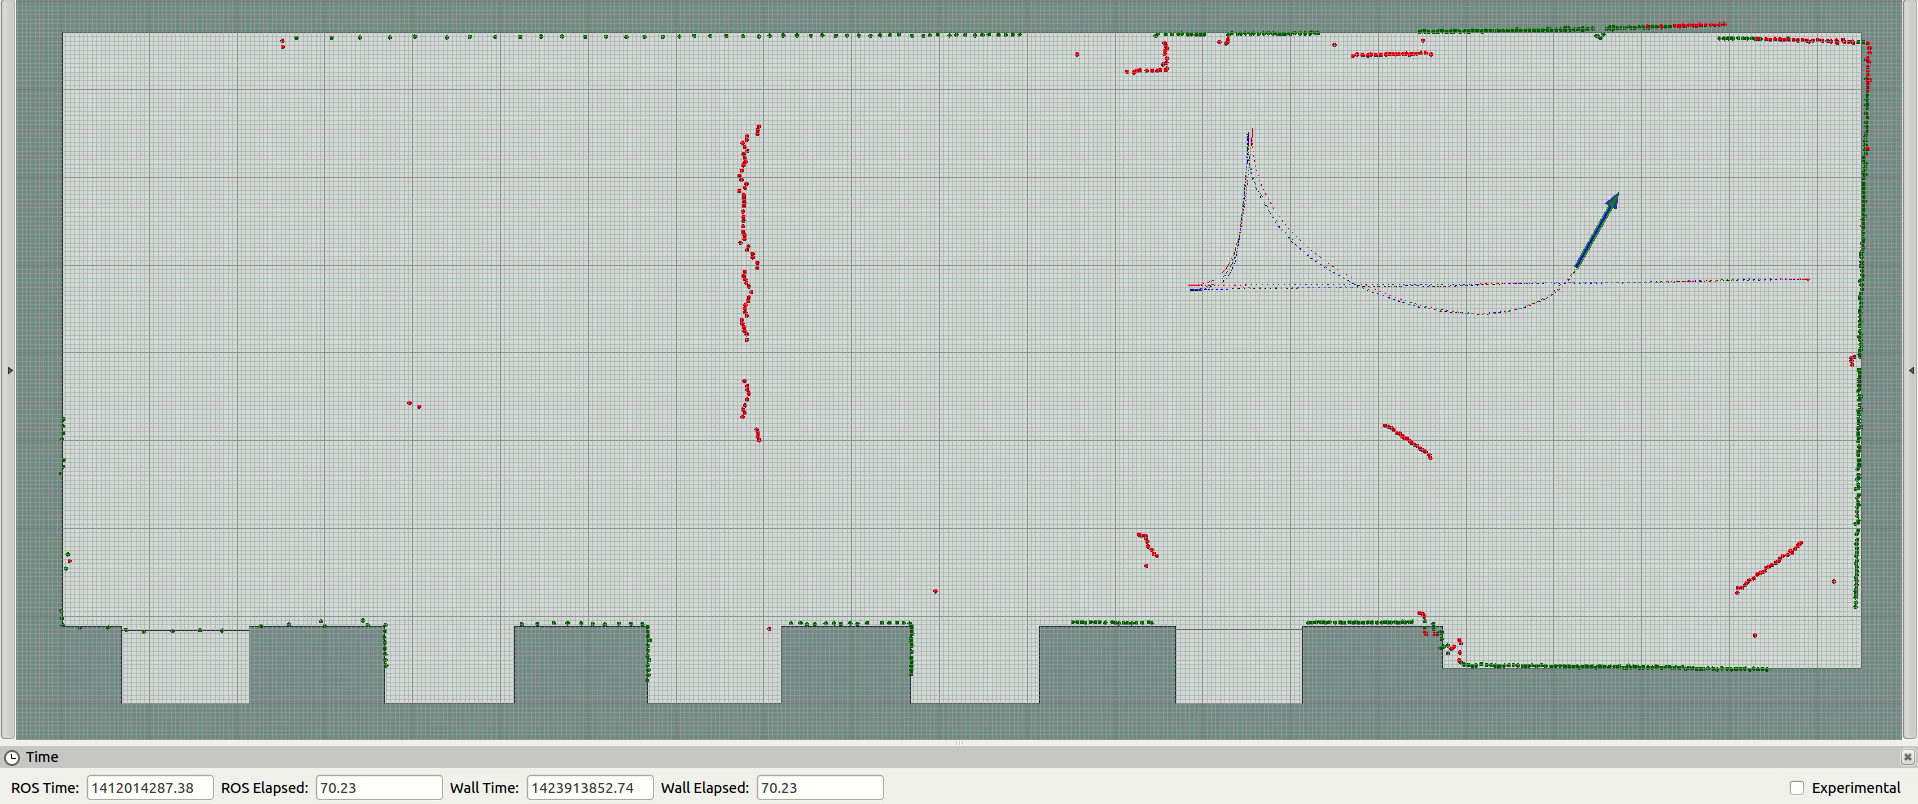
\includegraphics[width=0.97\textwidth]{localization-system-evaluation/tests-3dof/laser-spherical-interpolation/laser-deformation-2}
	\caption{Laser deformation when the robot is rotating}
	\label{fig:localization-system-evaluation_laser-deformation-2}
\end{figure}

\begin{figure}[H]
	\centering
	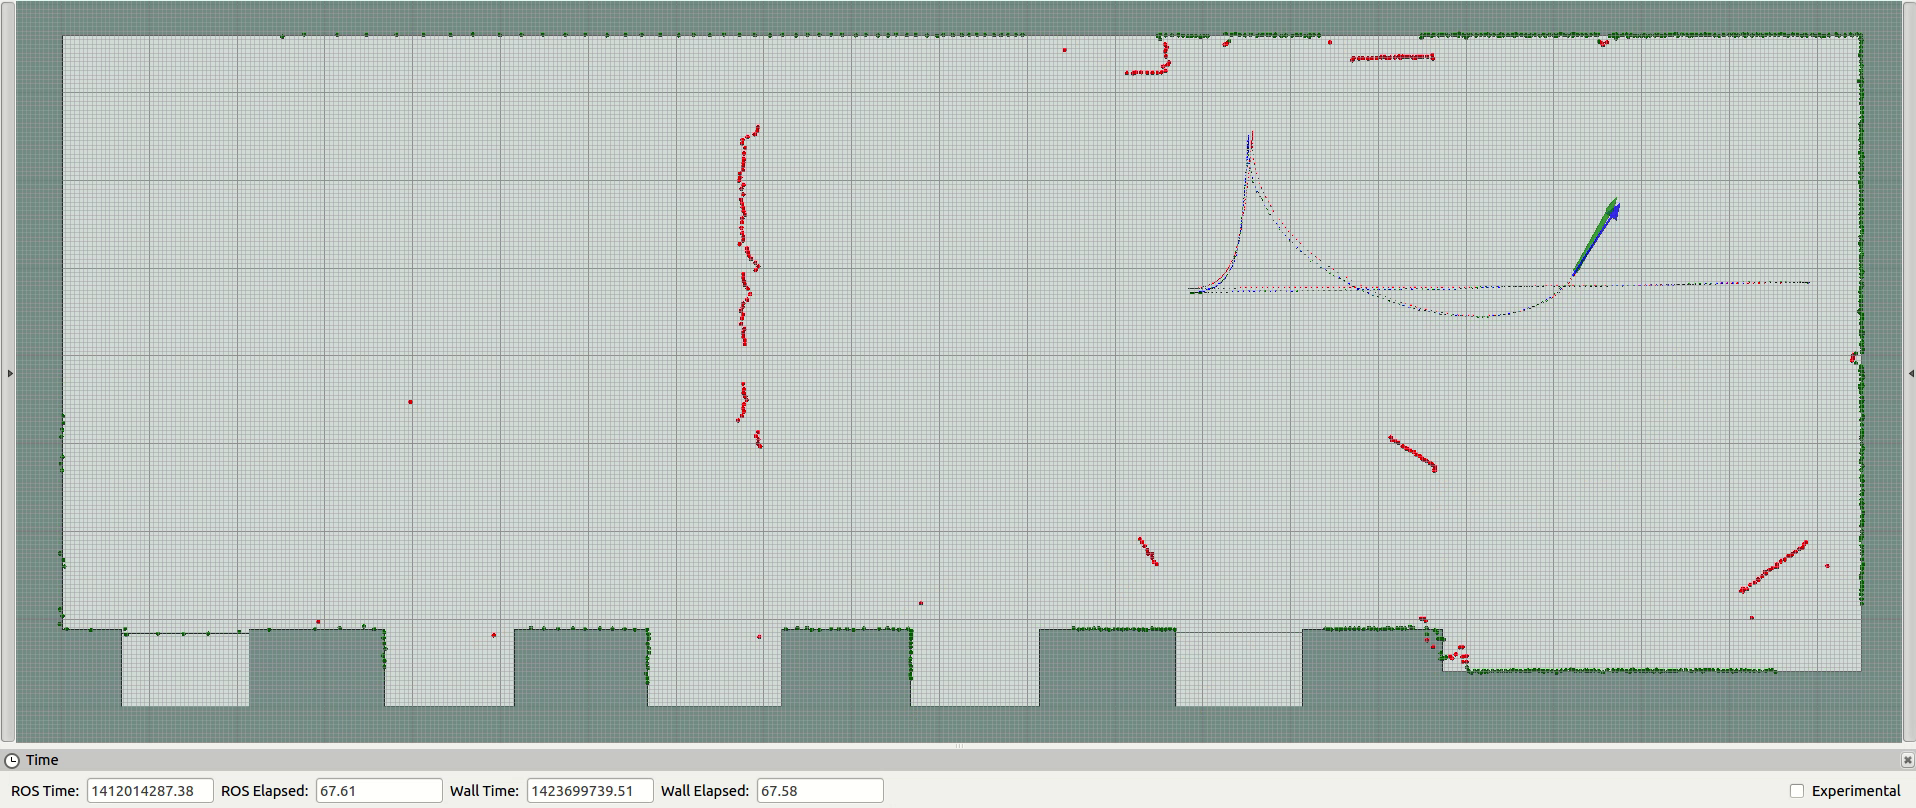
\includegraphics[width=0.97\textwidth]{localization-system-evaluation/tests-3dof/laser-spherical-interpolation/laser-deformation-2-corrected}
	\caption{Correction of the laser deformation with spherical linear interpolation}
	\label{fig:localization-system-evaluation_laser-deformation-2-corrected}
\end{figure}



\subsection{Point cloud preprocessing}

The statistical error of the lasers can be mitigated by merging several laser scans before performing a point cloud registration. This is based on the fact that a considerable amount of laser noise follows a Gaussian distribution, and as such, the effective measurement error can be significantly reduced by retrieving the centroids of a voxel grid applied over the laser data. However, assembling too much laser scans can lead to worse pose tracking if the robot is moving at high speeds, because the lasers would be projected into the map frame with a high position error (because odometry accuracy decreases when the robot speed increases and the localization system will not correct it). As such, the implemented laser assembler supports dynamic reconfiguration of the number of laser scans to assemble (or the period of assembly time) based on the robot estimated velocity. This feature besides improving the pose tracking, it also allows a navigation supervisor to regulate the rate at which the localization system operates. This can be very useful for mobile manipulators because the localization system can have a high update rate when the robot is moving fast and a low update rate when it is moving slower or when it is stopped. This allows a more efficient usage of the platform hardware resources while also improving the localization system accuracy.

Besides reducing the sensor measurement errors, this processing stage also allows the removal of laser shadow points caused by veiling, or small cluster of points that may be associated with temporary objects / people. Moreover, given that the time it takes to perform point cloud registration is proportional to the number of points in the reference and ambient point cloud, voxel / random downsampling can be a very effective technique to adjust the level of detail required (given the computational resources available).



\subsection{\glsentrytext{slam}}

Any self-localization system requires a map to estimate the pose of the robot when using exteroceptive information. If such map doesn't exist, then the first point cloud can be considered as the initial map, and then it can be updated dynamically as new sensor data is processed. This map update approach can use the full registered point cloud or the inliers / outliers only. Full integration is useful when starting a map from scratch (example in \cref{fig:localization-system-evaluation_drl-2.5cm-1.0-bag-speed}). Partial integration can be useful when there is a highly detailed map and we only want to add or remove information from it (examples from \crefrange{fig:localization-system-evaluation_lab-10mm}{fig:localization-system-evaluation_indoor-10mm-dynamic}). Partial integration besides reducing the computational resources required it also allows to keep the detail of the source map, avoiding deformations due to sensor measurement noise. This noise is noticeable in the map in \cref{fig:localization-system-evaluation_lab-10mm-dynamic} (updated with full integration) and was avoided in the map in \cref{fig:localization-system-evaluation_indoor-10mm-dynamic} (updated with outliers only).

Looking at figures from \crefrange{fig:localization-system-evaluation_drl-2.5cm-1.0-bag-speed}{fig:localization-system-evaluation_ground-truth-2.5cm-0.245-time-offset} it can be seen that the proposed localization system was able to achieve equal or even better mapping results than the GMapping\footnote{\url{http://wiki.ros.org/gmapping}} \gls{slam} system and even the ground truth provided by the Raptor-E cameras (that seems to be less suitable for mapping than both the proposed localization system and the GMapping \gls{ros} package).


\begin{figure}[H]
	\centering
	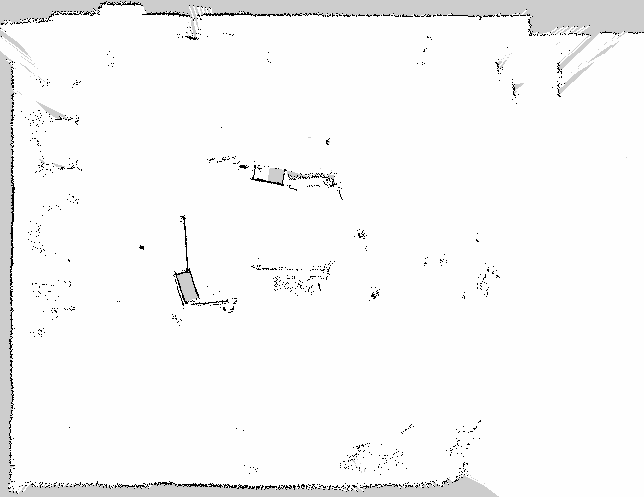
\includegraphics[width=0.53\textwidth]{localization-system-evaluation/tests-3dof/maps/industrial-hall/drl-2.5cm-1.0-bag-speed}
	\caption{Map made with the localization system using full integration in conjunction with OctoMap}
	\label{fig:localization-system-evaluation_drl-2.5cm-1.0-bag-speed}
\end{figure}

\begin{figure}[H]
	\centering
	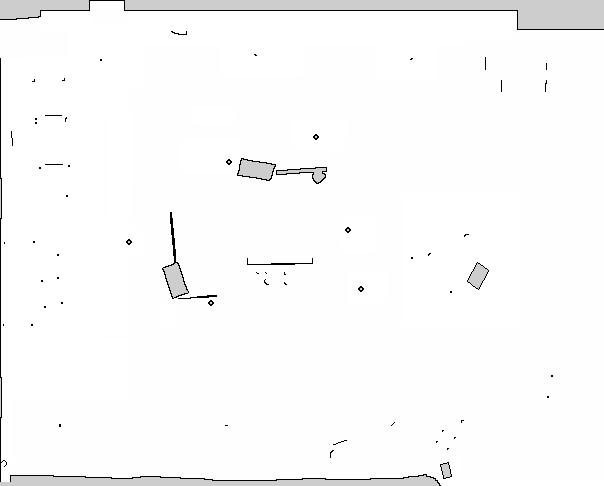
\includegraphics[width=0.53\textwidth]{localization-system-evaluation/tests-3dof/maps/industrial-hall/drl_corrected}
	\caption{Map manually corrected using the previous figure as starting point}
	\label{fig:localization-system-evaluation_drl_corrected}
\end{figure}

\begin{figure}[H]
	\centering
	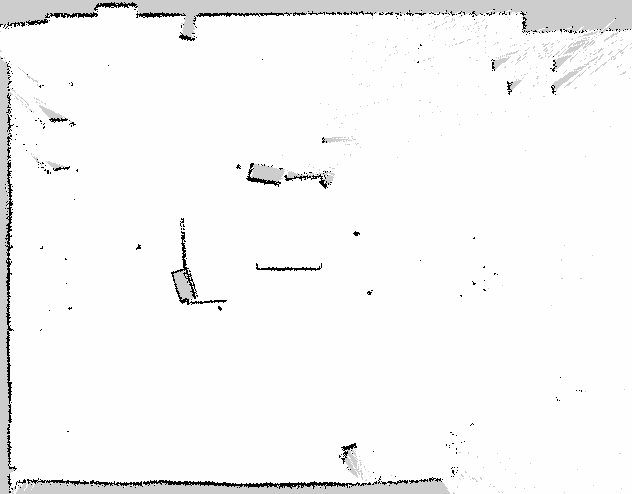
\includegraphics[width=0.53\textwidth]{localization-system-evaluation/tests-3dof/maps/industrial-hall/gmapping-2.5cm-0.1-bag-speed}
	\caption{Map made with the GMapping package playing the rosbag at 10\% speed}
	\label{fig:localization-system-evaluation_gmapping-2.5cm-0.1-bag-speed}
\end{figure}

\begin{figure}[H]
	\centering
	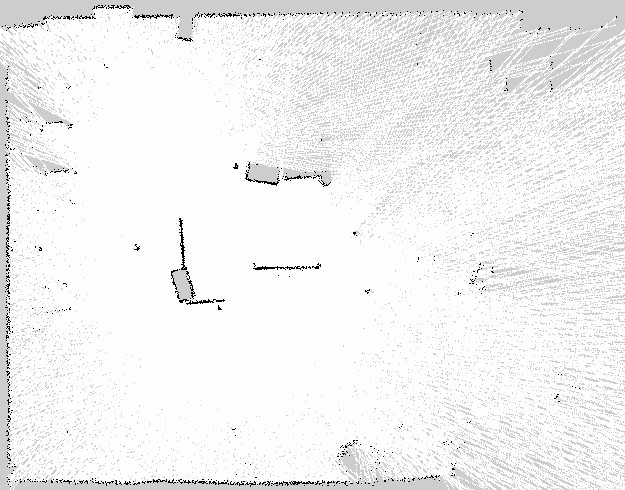
\includegraphics[width=0.65\textwidth]{localization-system-evaluation/tests-3dof/maps/industrial-hall/gmapping-2.5cm-1.0-bag-speed}
	\caption{Map made with the GMapping package playing the rosbag in real time}
	\label{fig:localization-system-evaluation_gmapping-2.5cm-1.0-bag-speed}
\end{figure}

\begin{figure}[H]
	\centering
	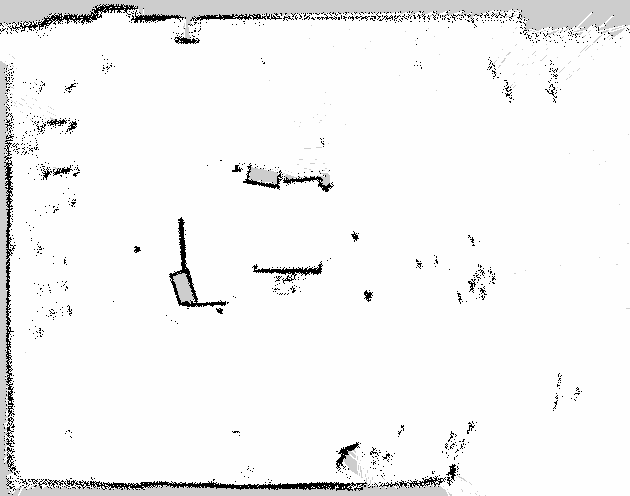
\includegraphics[width=0.65\textwidth]{localization-system-evaluation/tests-3dof/maps/industrial-hall/ground-truth-2.5cm-0.245-time-offset}
	\caption{Map made using the ground truth poses provided by the Raptor-E cameras}
	\label{fig:localization-system-evaluation_ground-truth-2.5cm-0.245-time-offset}
\end{figure}


\begin{figure}[H]
	\centering
	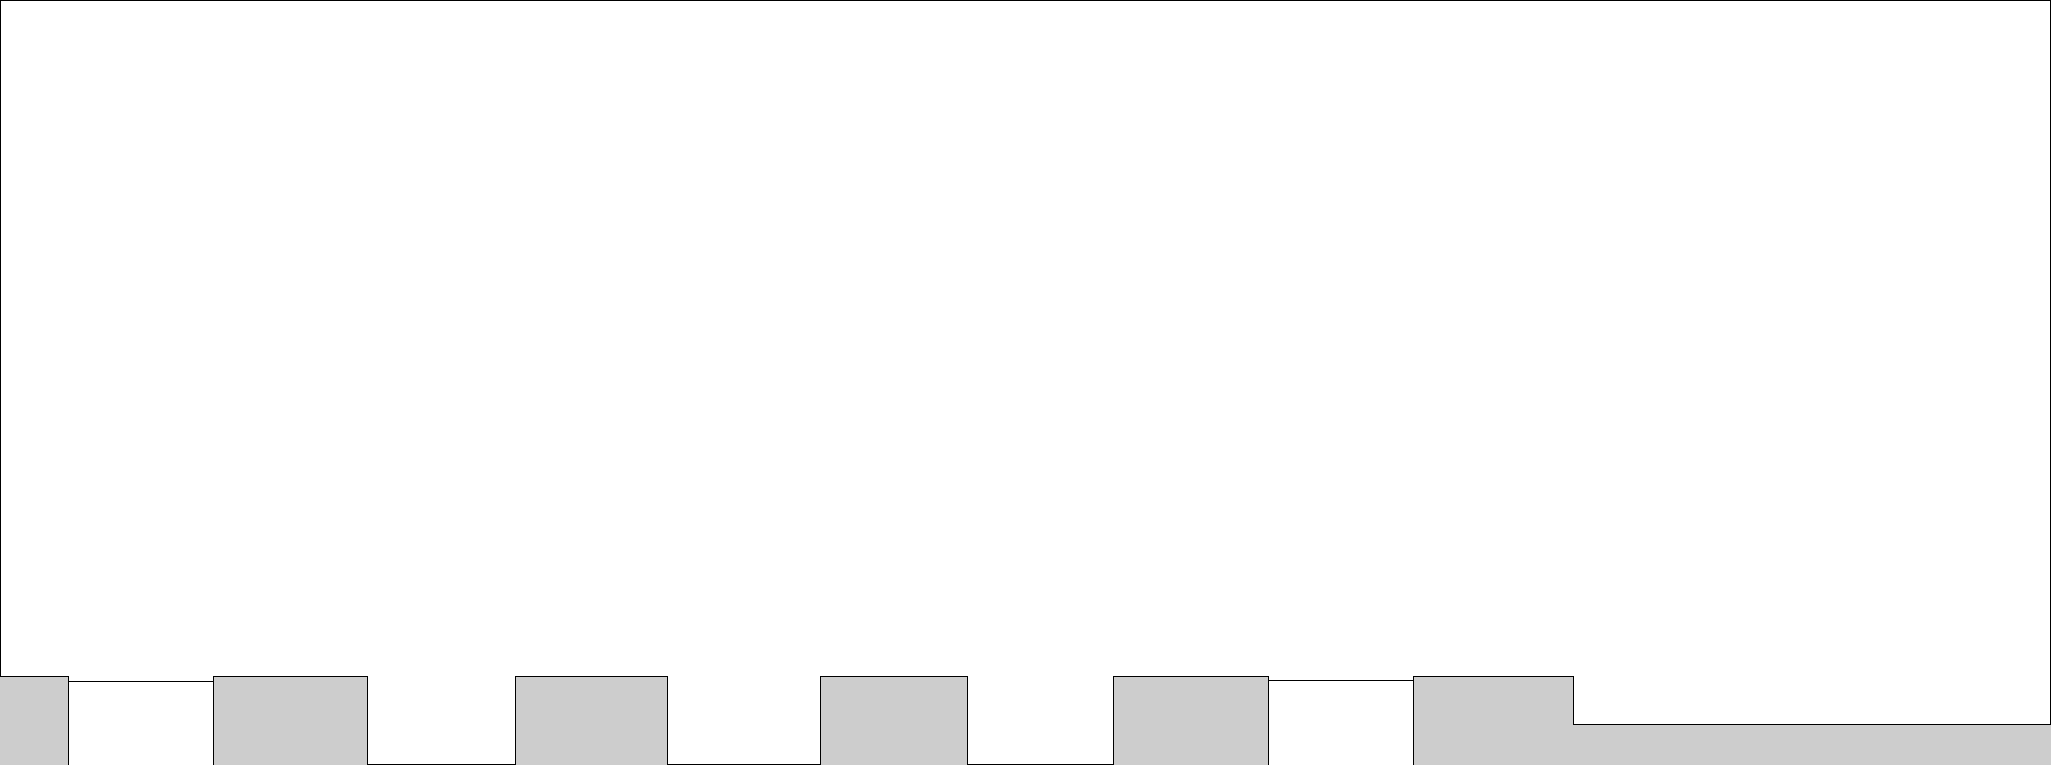
\includegraphics[width=0.7\textwidth]{localization-system-evaluation/tests-3dof/maps/lab-10mm}
	\caption{Original map from room i-108}
	\label{fig:localization-system-evaluation_lab-10mm}
\end{figure}

\begin{figure}[H]
	\centering
	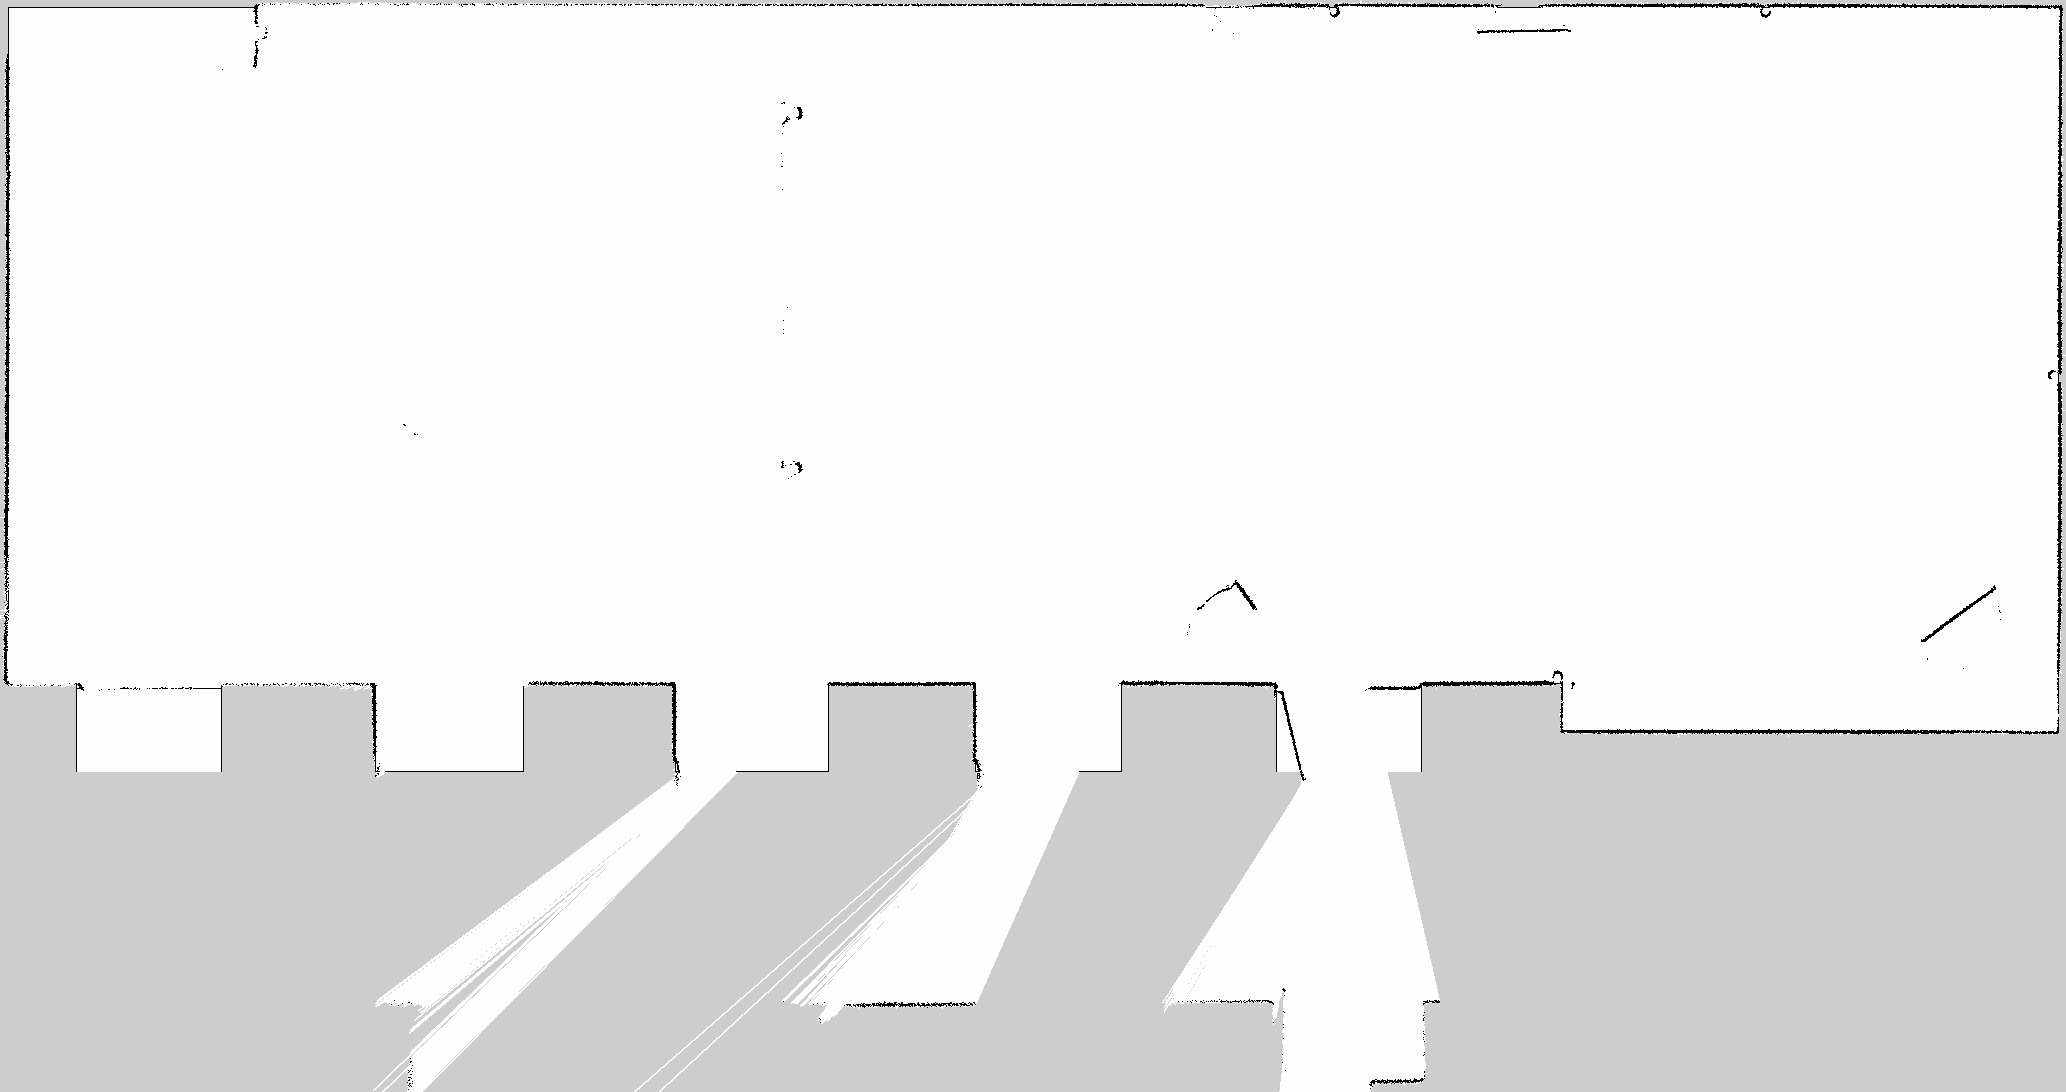
\includegraphics[width=0.7\textwidth]{localization-system-evaluation/tests-3dof/maps/lab-10mm-dynamic}
	\caption{Updated map of room i-108 using full integration}
	\label{fig:localization-system-evaluation_lab-10mm-dynamic}
\end{figure}

\begin{figure}[H]
	\centering
	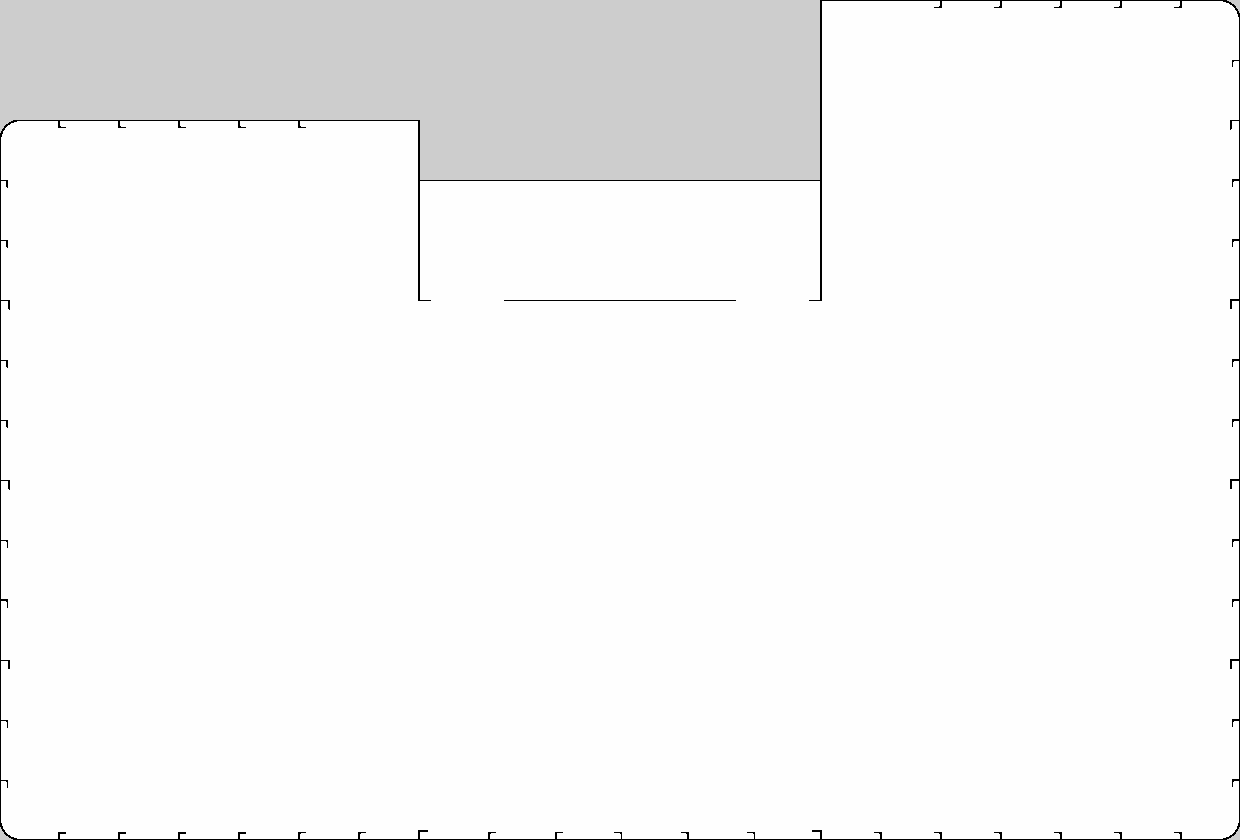
\includegraphics[width=0.67\textwidth]{localization-system-evaluation/tests-3dof/maps/indoor-10mm}
	\caption{Original map of structured environment}
	\label{fig:localization-system-evaluation_indoor-10mm}
\end{figure}

\begin{figure}[H]
	\centering
	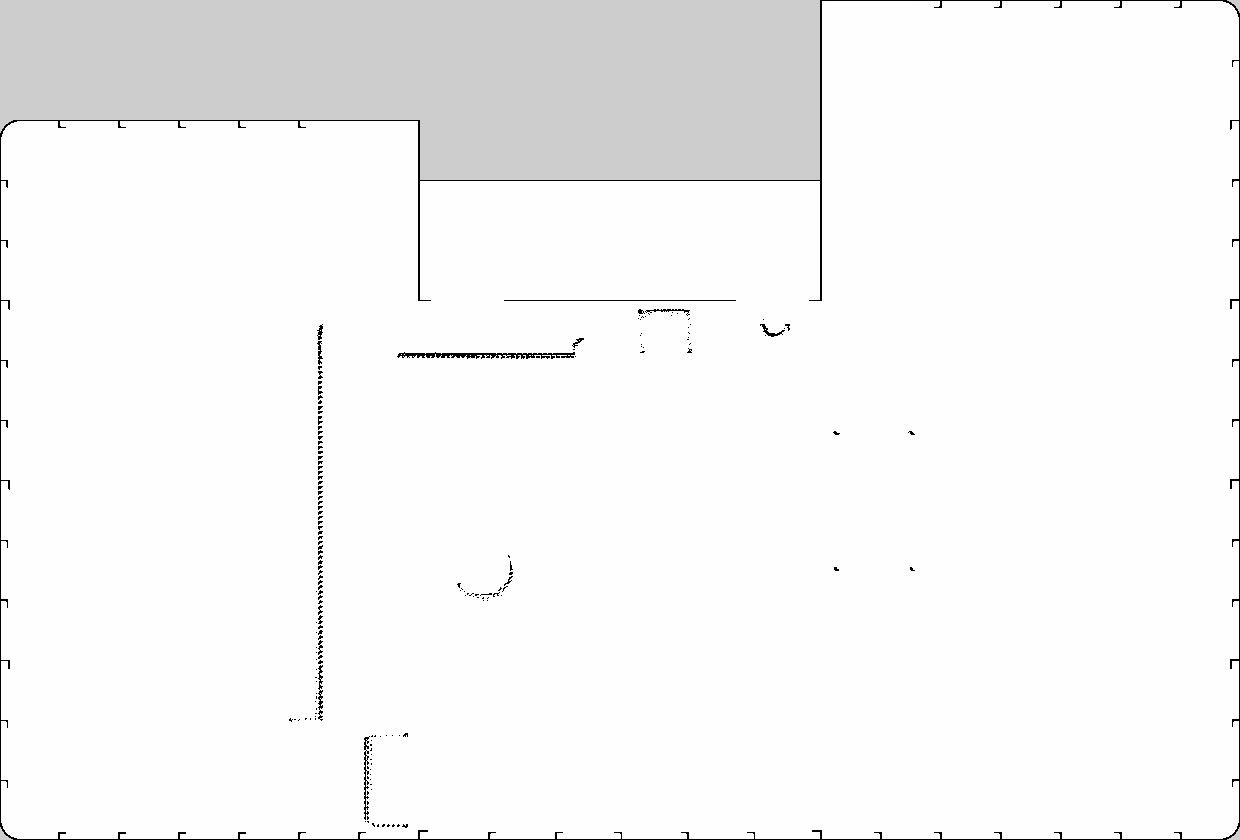
\includegraphics[width=0.67\textwidth]{localization-system-evaluation/tests-3dof/maps/indoor-10mm-dynamic}
	\caption{Updated map of structured environment using partial integration (outliers)}
	\label{fig:localization-system-evaluation_indoor-10mm-dynamic}
\end{figure}



\subsection{Point cloud registration}

Looking at the results present in \cref{app:appendix-a}, such as the laser assembly figures and translation / rotation error graphs from the Jarvis test in the complex path at high velocities (shown from \crefrange{fig:localization-system-evaluation_complex-path-with-outliers-50-30-50-10cm-per-sec-velocity-1-4-scans-drl-cumulative}{fig:localization-system-evaluation_complex-path-with-outliers-50-30-50-10cm-per-sec-velocity-1-4-rotation-error}), it can be seen that the localization system can registered point clouds with much more accuracy than \gls{amcl} (even when using over 5000 particles). The only problems that seem to affect the used algorithms are the point cloud deformation (usually when there is unreliable odometry information, which typically occurs when the robot is moving with high velocities / accelerations), laser measurements errors, unknown objects close to the known reference point cloud and also low resolution maps.

The localization system can tolerate these problems by having a default pipeline configuration for the normal operation of the robot, another for temporary tracking recovery and yet another for initial pose estimation.

The switch between the localization system operation modes using the point cloud registration analysis proved to be a very intuitive and fast process and the overall system configurations seemed to be generic enough to be reused in several types of environments, with different robots equipped with varying types of sensors. Such ease of configuration allows the fast deployment of robots and gives a high confidence that the localization system will remain accurate even in challenging environments. This is not the case with systems such as \gls{amcl}, given that they are very dependent on the odometry and laser models, and as such, require constant retuning when one of these models change.

The ability to switch registration algorithms at runtime based on the quality of the estimated pose proved to be an efficient and flexible architecture choice, since it allowed high precision pose tracking with fast registration algorithms and occasional pose tracking recovery with more robust methods (which happened more often in the tests at higher velocities, in which the odometry was significantly worse).

The initial pose estimation using feature matching was very reliable and successfully found the robot location even in low feature surroundings (as can be seen from \crefrange{fig:localization-system-evaluation_ship-interior-initial-pose-estimation-sift-fpfh-ransac-gicp}{fig:localization-system-evaluation_jarvis-initial-pose-estimation-sift-fpfh-ransac-gicp-2}). Moreover, the output of the accepted initial pose estimations allows the detection of similar map locations by a navigation supervisor, which can then plot a path to disambiguate the initial pose guess and avoid dangerous operations at a wrong position.

\Crefrange{fig:localization-system-evaluation_ship-interior-initial-pose-estimation-sift-fpfh-ransac-gicp}{fig:localization-system-evaluation_jarvis-initial-pose-estimation-sift-fpfh-ransac-gicp-1} show the accepted initial pose estimations using the global localization subsystem presented in \cref{subsec:localization-system_feature-registration}.

The blue circles presented in \cref{fig:localization-system-evaluation_jarvis-initial-pose-estimation-sift-fpfh-ransac-gicp-1} represent the keypoints of the ambient point cloud in the robot start up position, while the violet circles are the reference point cloud keypoints. The green circles are the ambient point cloud laser measurements after performing the initial pose estimation and registration refinement.



\begin{figure}[H]
	\centering
	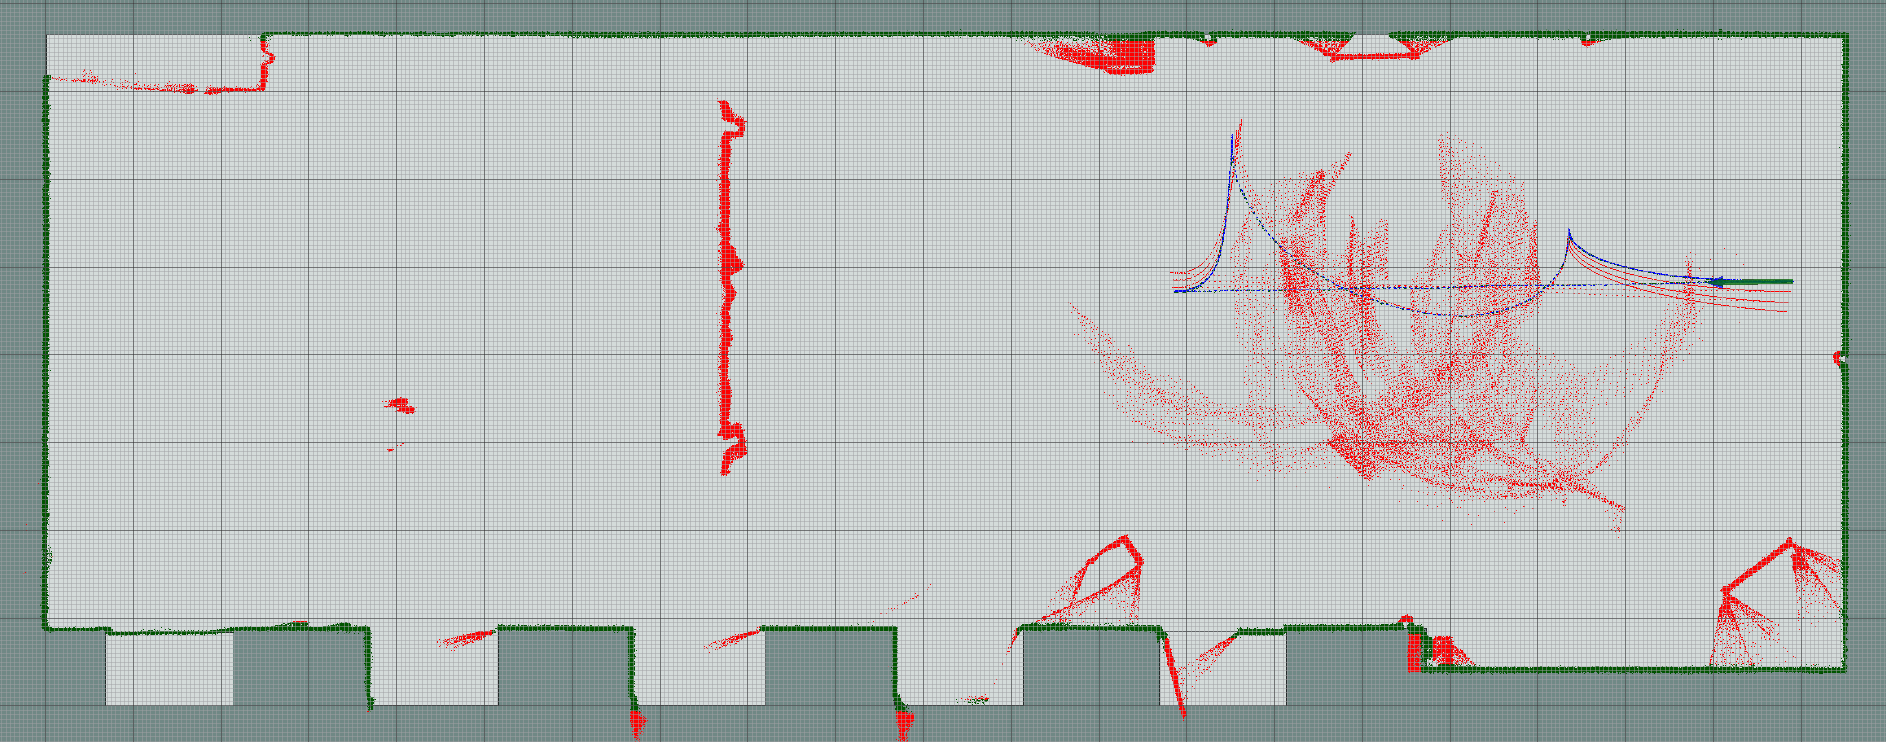
\includegraphics[width=0.997\textwidth]{appendices/tests-3dof/jarvis-robot/complex-path-with-outliers-50-30-50-10cm-per-sec-velocity-1-4-scans/drl-cumulative}
	\caption{Laser scans assembled on top of the map using the localization system poses}
	\label{fig:localization-system-evaluation_complex-path-with-outliers-50-30-50-10cm-per-sec-velocity-1-4-scans-drl-cumulative}
\end{figure}

\begin{figure}[H]
	\centering
	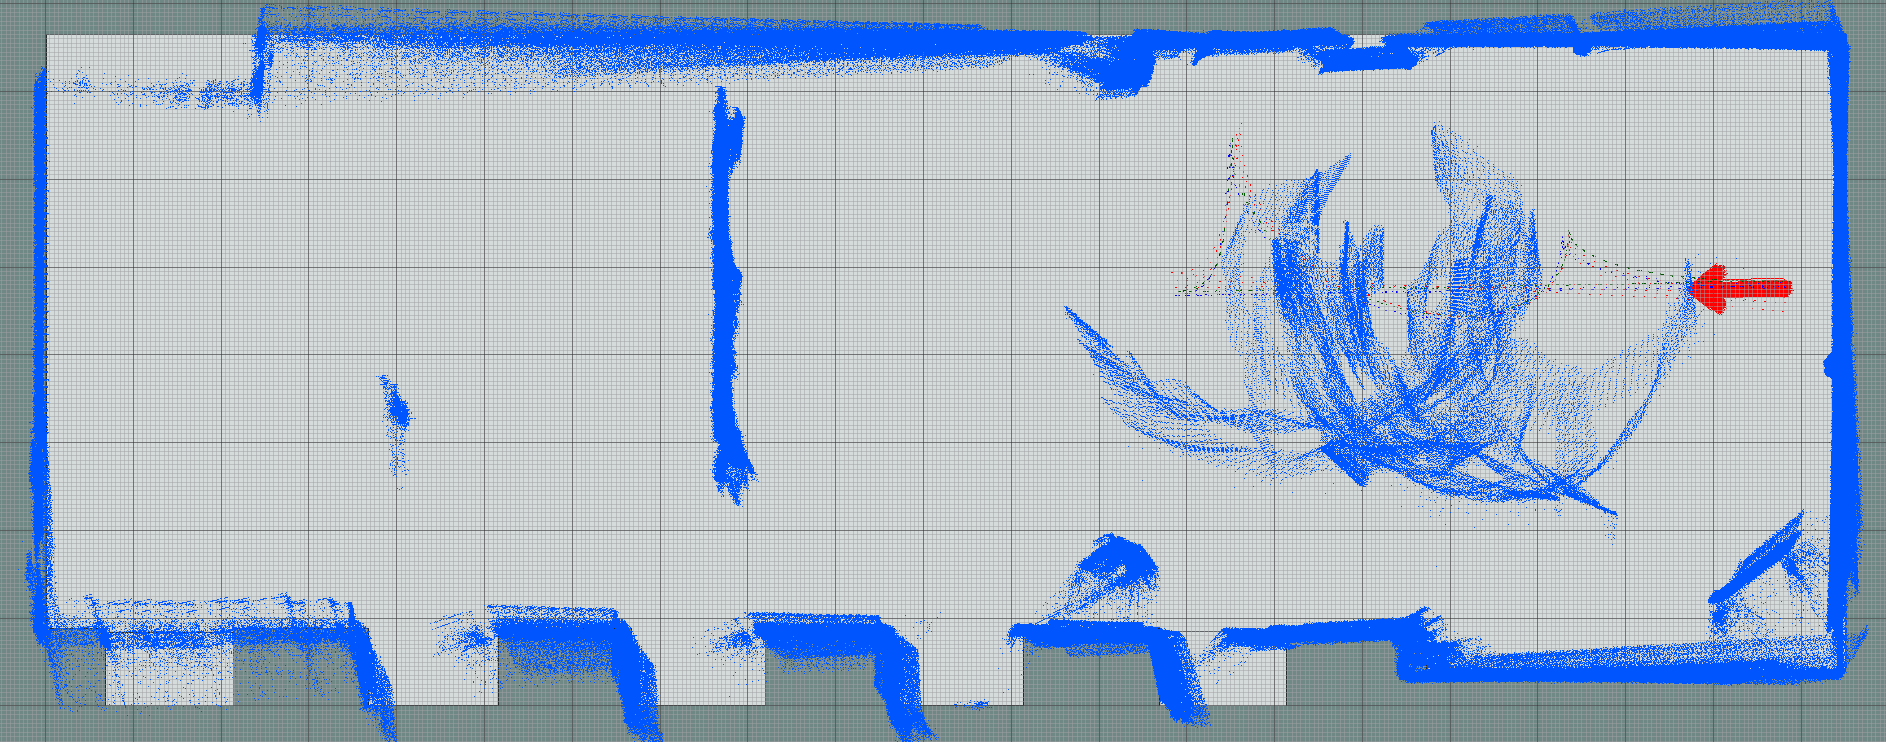
\includegraphics[width=0.997\textwidth]{appendices/tests-3dof/jarvis-robot/complex-path-with-outliers-50-30-50-10cm-per-sec-velocity-1-4-scans/amcl-cumulative}
	\caption{Laser scans assembled on top of the map using the \glsentrytext{amcl} poses}
	\label{fig:localization-system-evaluation_complex-path-with-outliers-50-30-50-10cm-per-sec-velocity-1-4-scans-amcl-cumulative}
\end{figure}


\begin{figure}
	\centering
	\begin{minipage}[h]{0.497\textwidth}
		\centering
		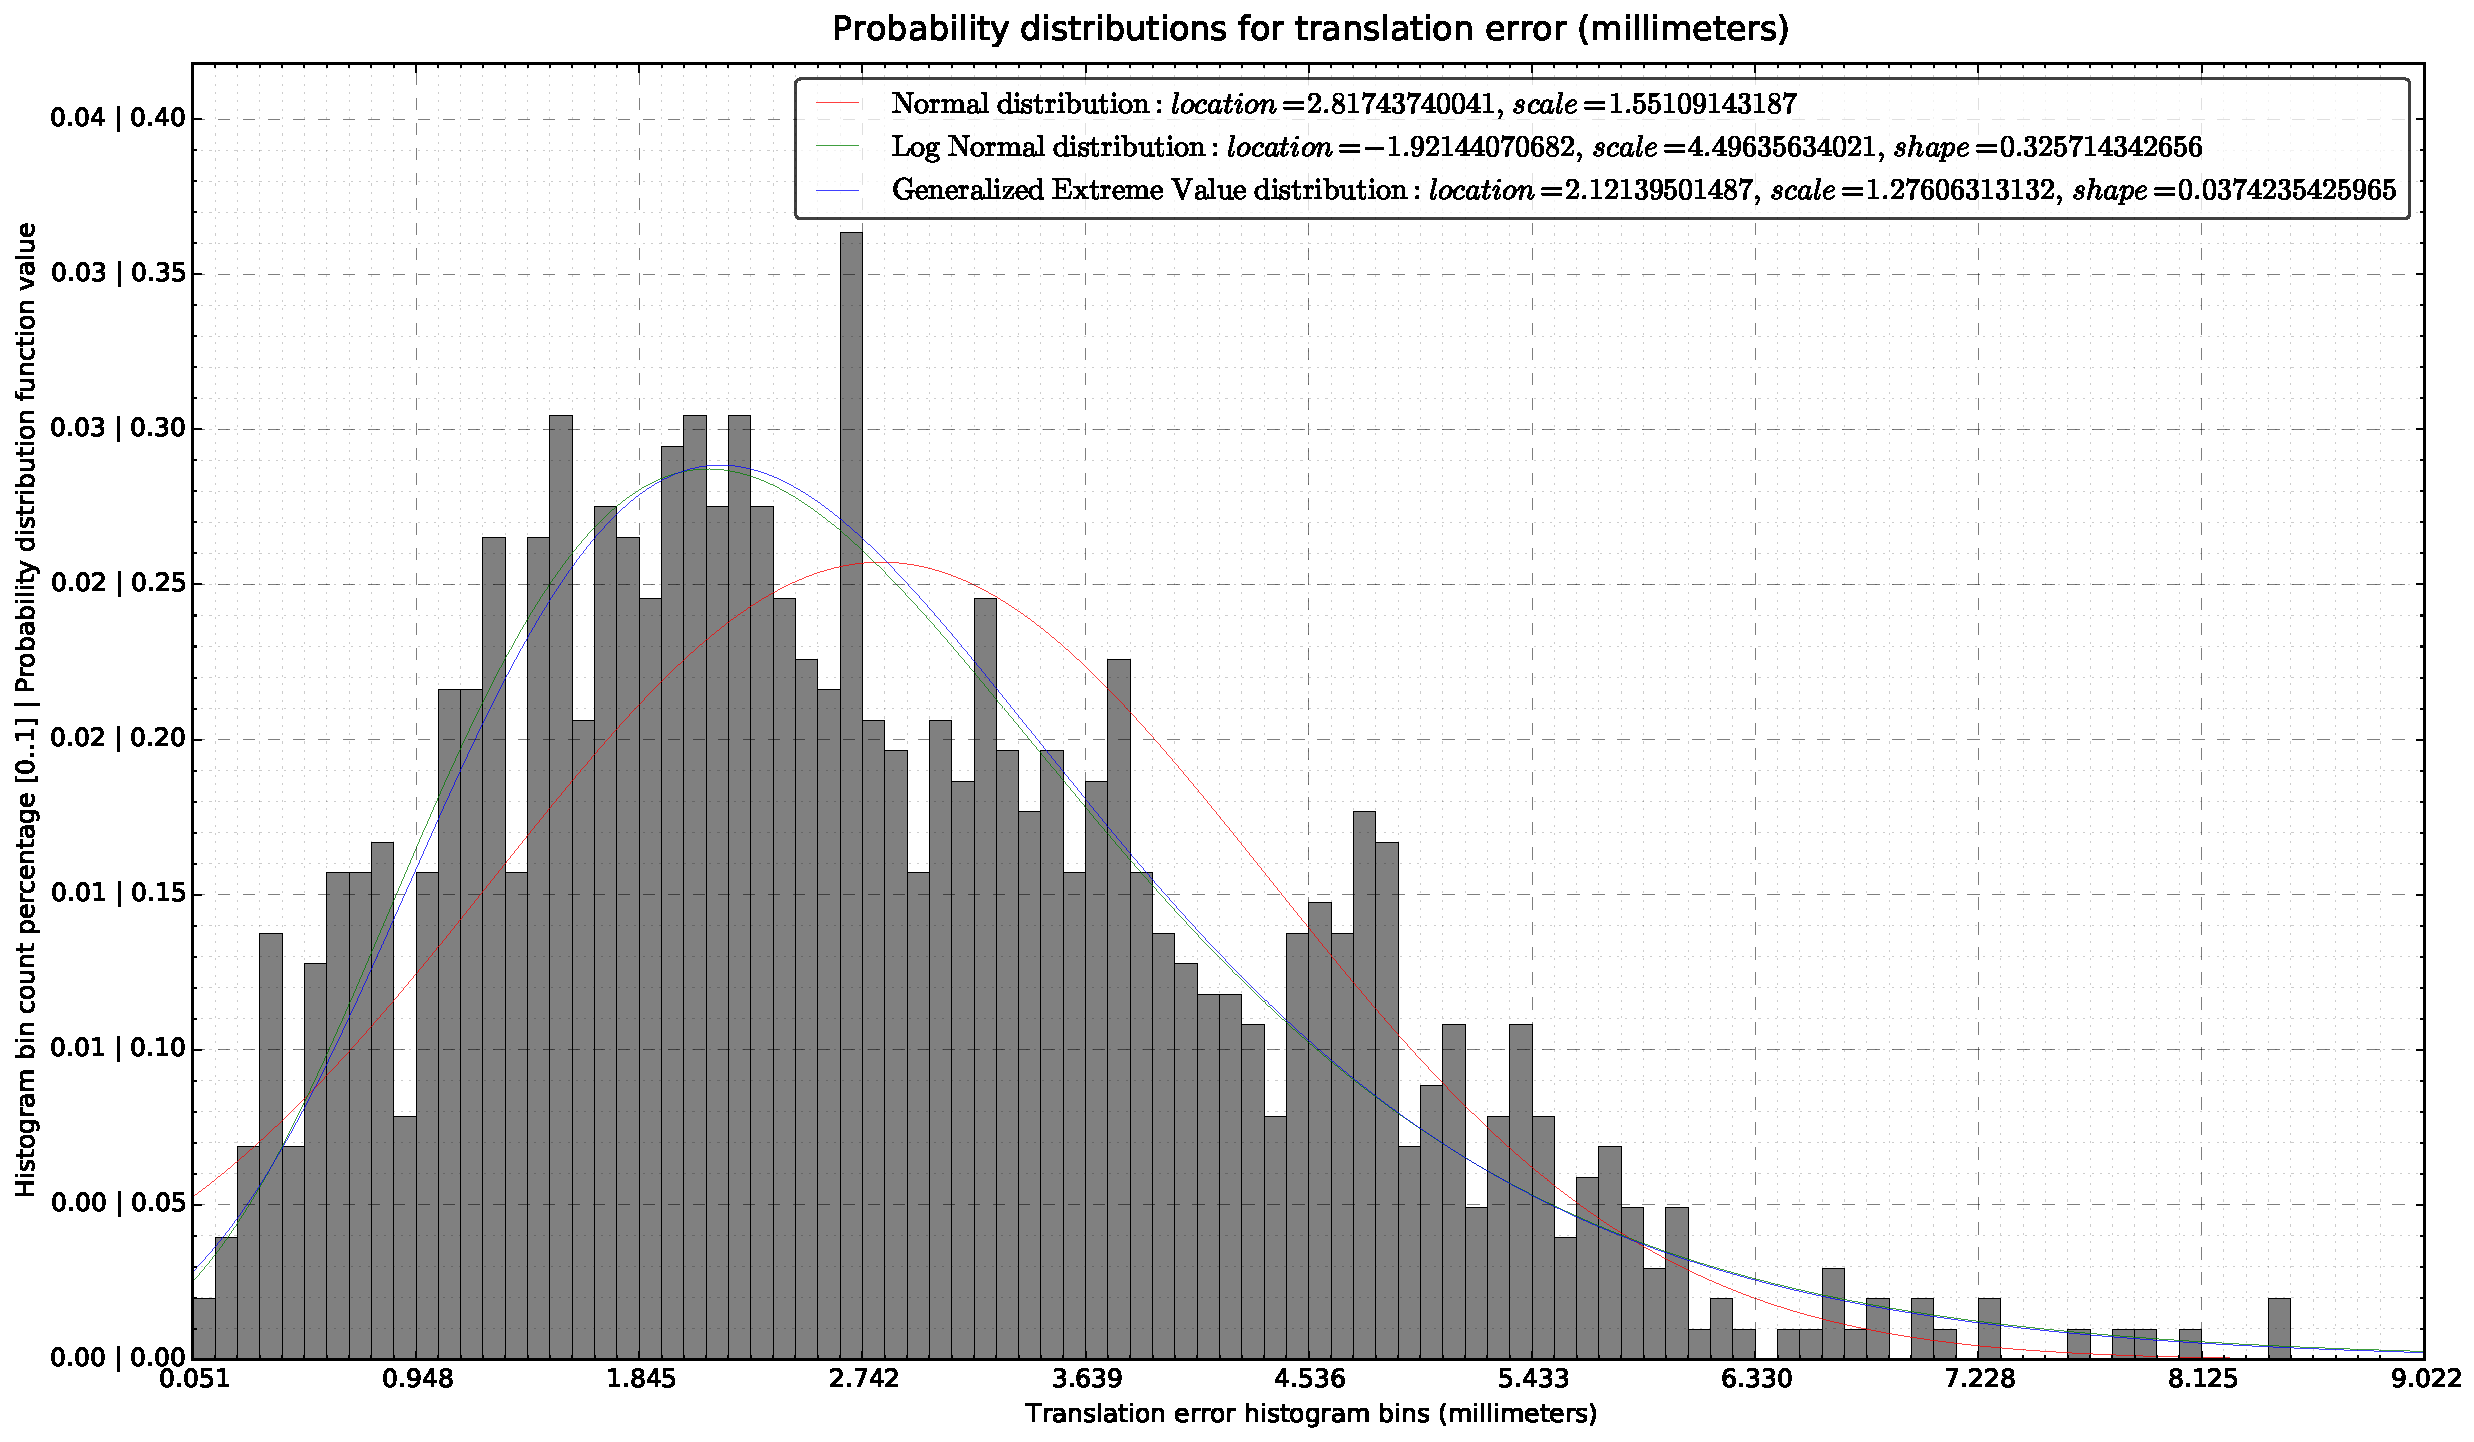
\includegraphics[width=0.997\textwidth]{appendices/tests-3dof/jarvis-robot/complex-path-with-outliers-50-30-50-10cm-per-sec-velocity-1-4-scans/graphs/translation-error-millimeters-distributions}
		\caption{Probability distributions for the localization system translation errors}
		\label{fig:localization-system-evaluation_complex-path-with-outliers-50-30-50-10cm-per-sec-velocity-1-4-translation-error}
	\end{minipage}\hfill
	\begin{minipage}[h]{0.497\textwidth}
		\centering
		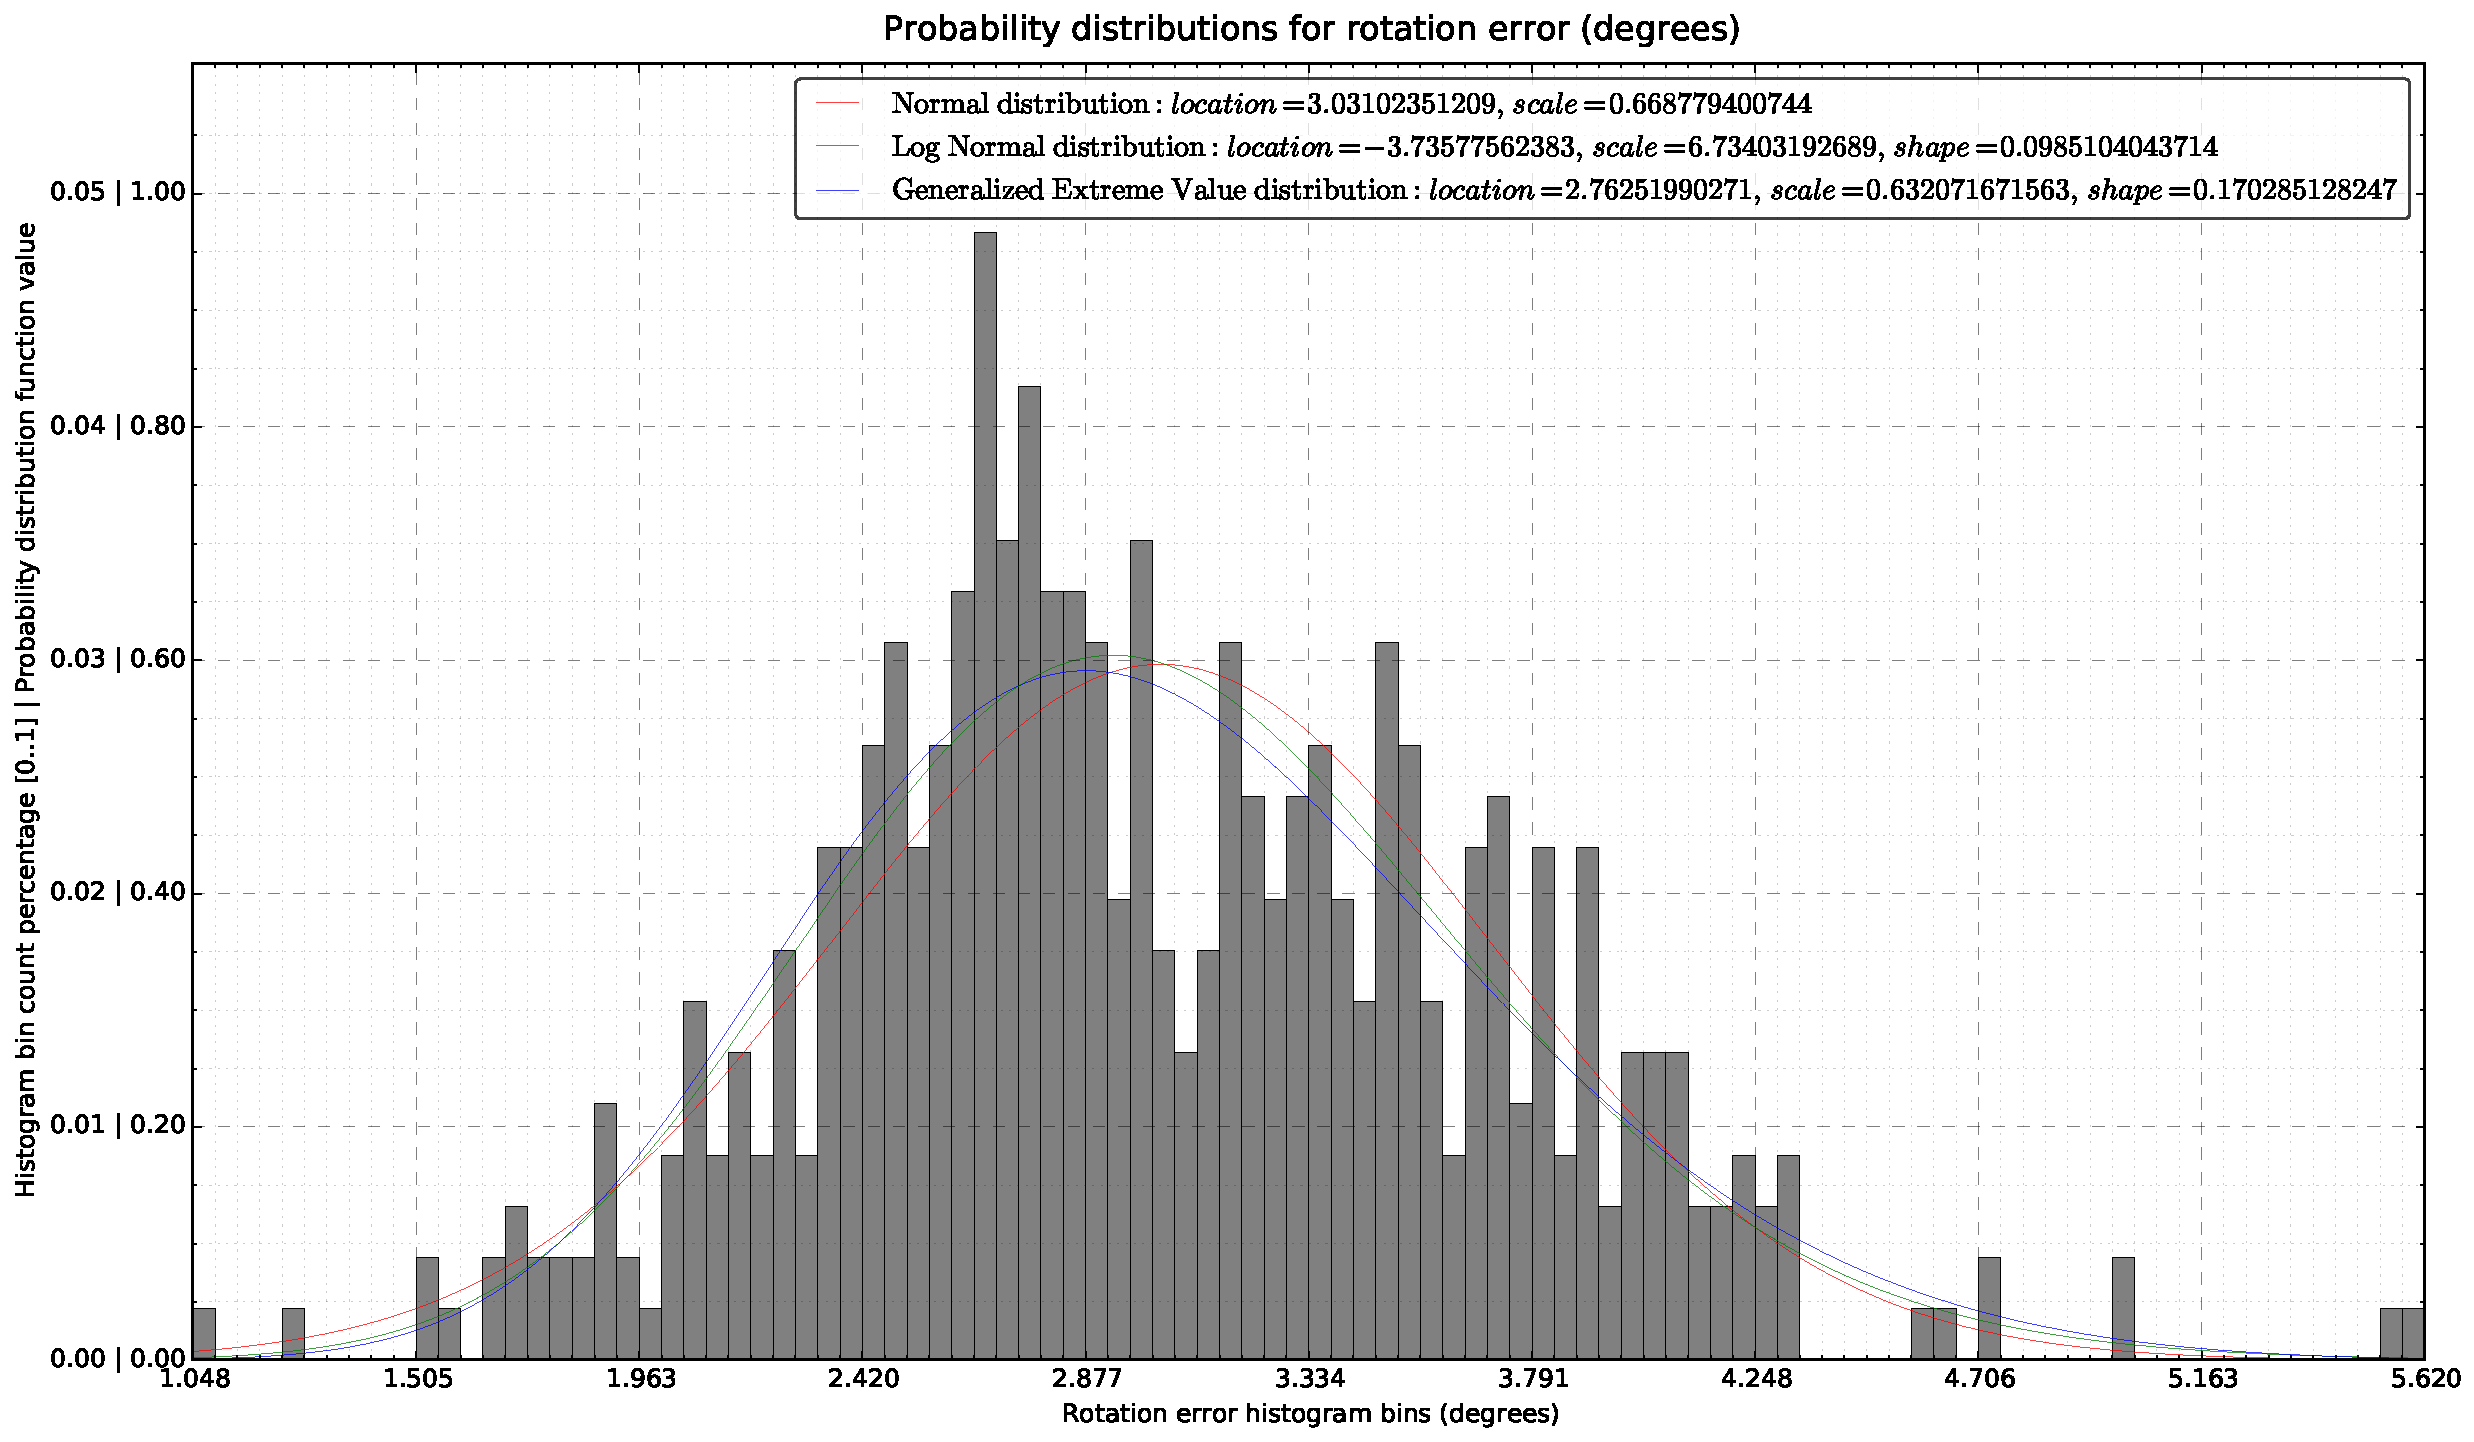
\includegraphics[width=0.997\textwidth]{appendices/tests-3dof/jarvis-robot/complex-path-with-outliers-50-30-50-10cm-per-sec-velocity-1-4-scans/graphs/rotation-error-degrees-distributions}
		\caption{Probability distributions for the localization system rotation errors}
		\label{fig:localization-system-evaluation_complex-path-with-outliers-50-30-50-10cm-per-sec-velocity-1-4-rotation-error}
	\end{minipage}
\end{figure}


\begin{figure}[H]
	\centering
	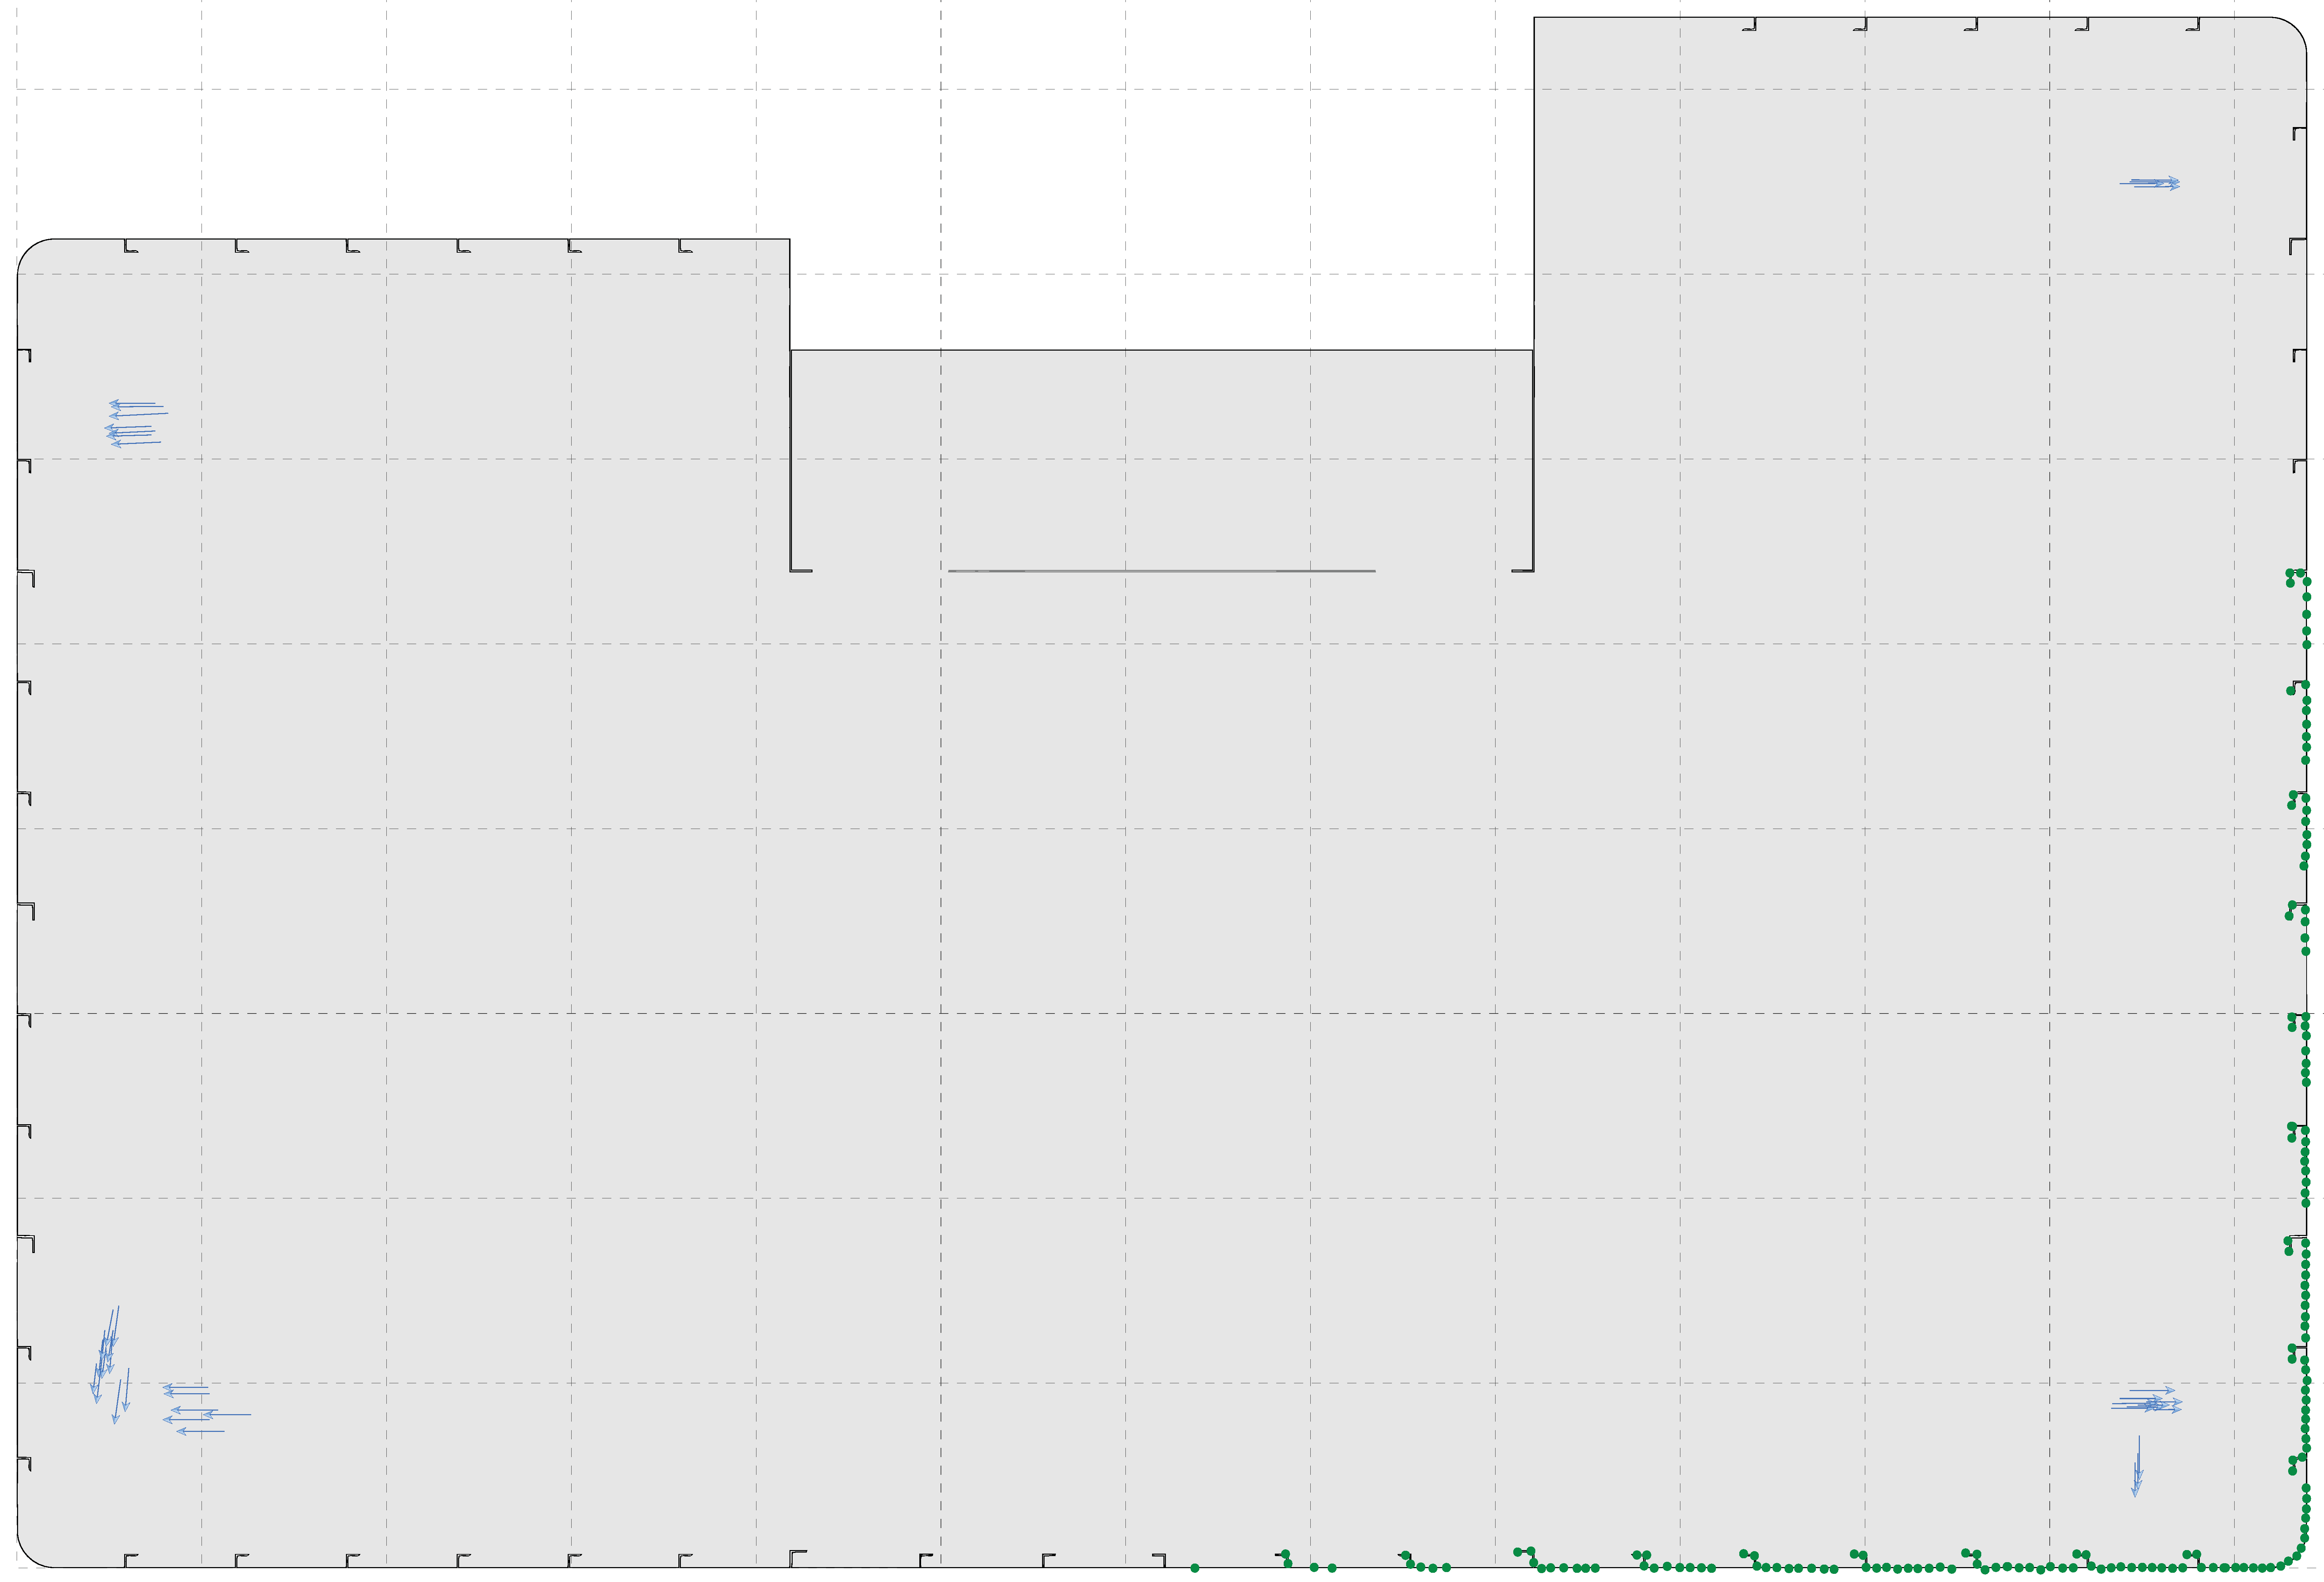
\includegraphics[width=0.87\textwidth]{localization-system-evaluation/tests-3dof/initial_pose_estimation/ship-interior-initial-pose-estimation-sift-fpfh-ransac-gicp}
	\caption{Initial pose estimation using feature matching in Guardian static environment}
	\label{fig:localization-system-evaluation_ship-interior-initial-pose-estimation-sift-fpfh-ransac-gicp}
\end{figure}

\begin{figure}[H]
	\centering
	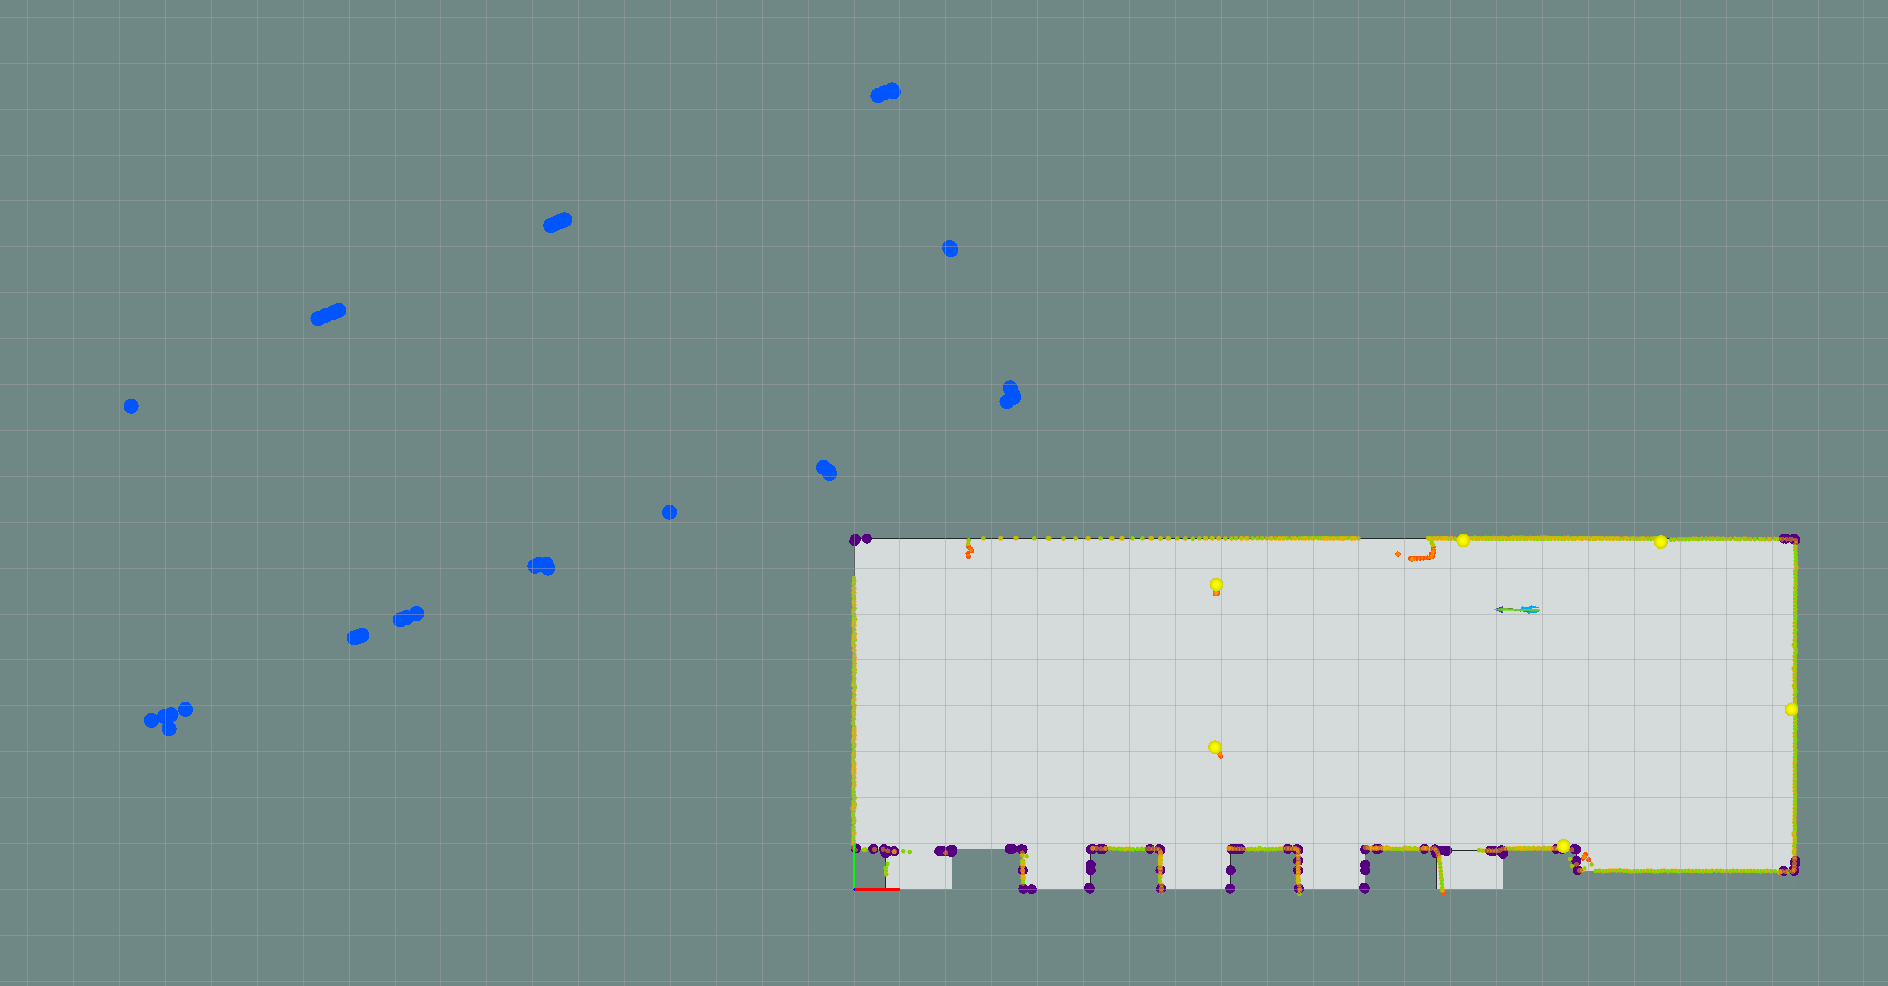
\includegraphics[width=0.87\textwidth]{localization-system-evaluation/tests-3dof/initial_pose_estimation/jarvis-initial-pose-estimation-sift-fpfh-ransac-gicp-1}
	\caption{Initial pose estimation using feature matching in Jarvis environment}
	\label{fig:localization-system-evaluation_jarvis-initial-pose-estimation-sift-fpfh-ransac-gicp-1}
\end{figure}

\begin{figure}[H]
	\centering
	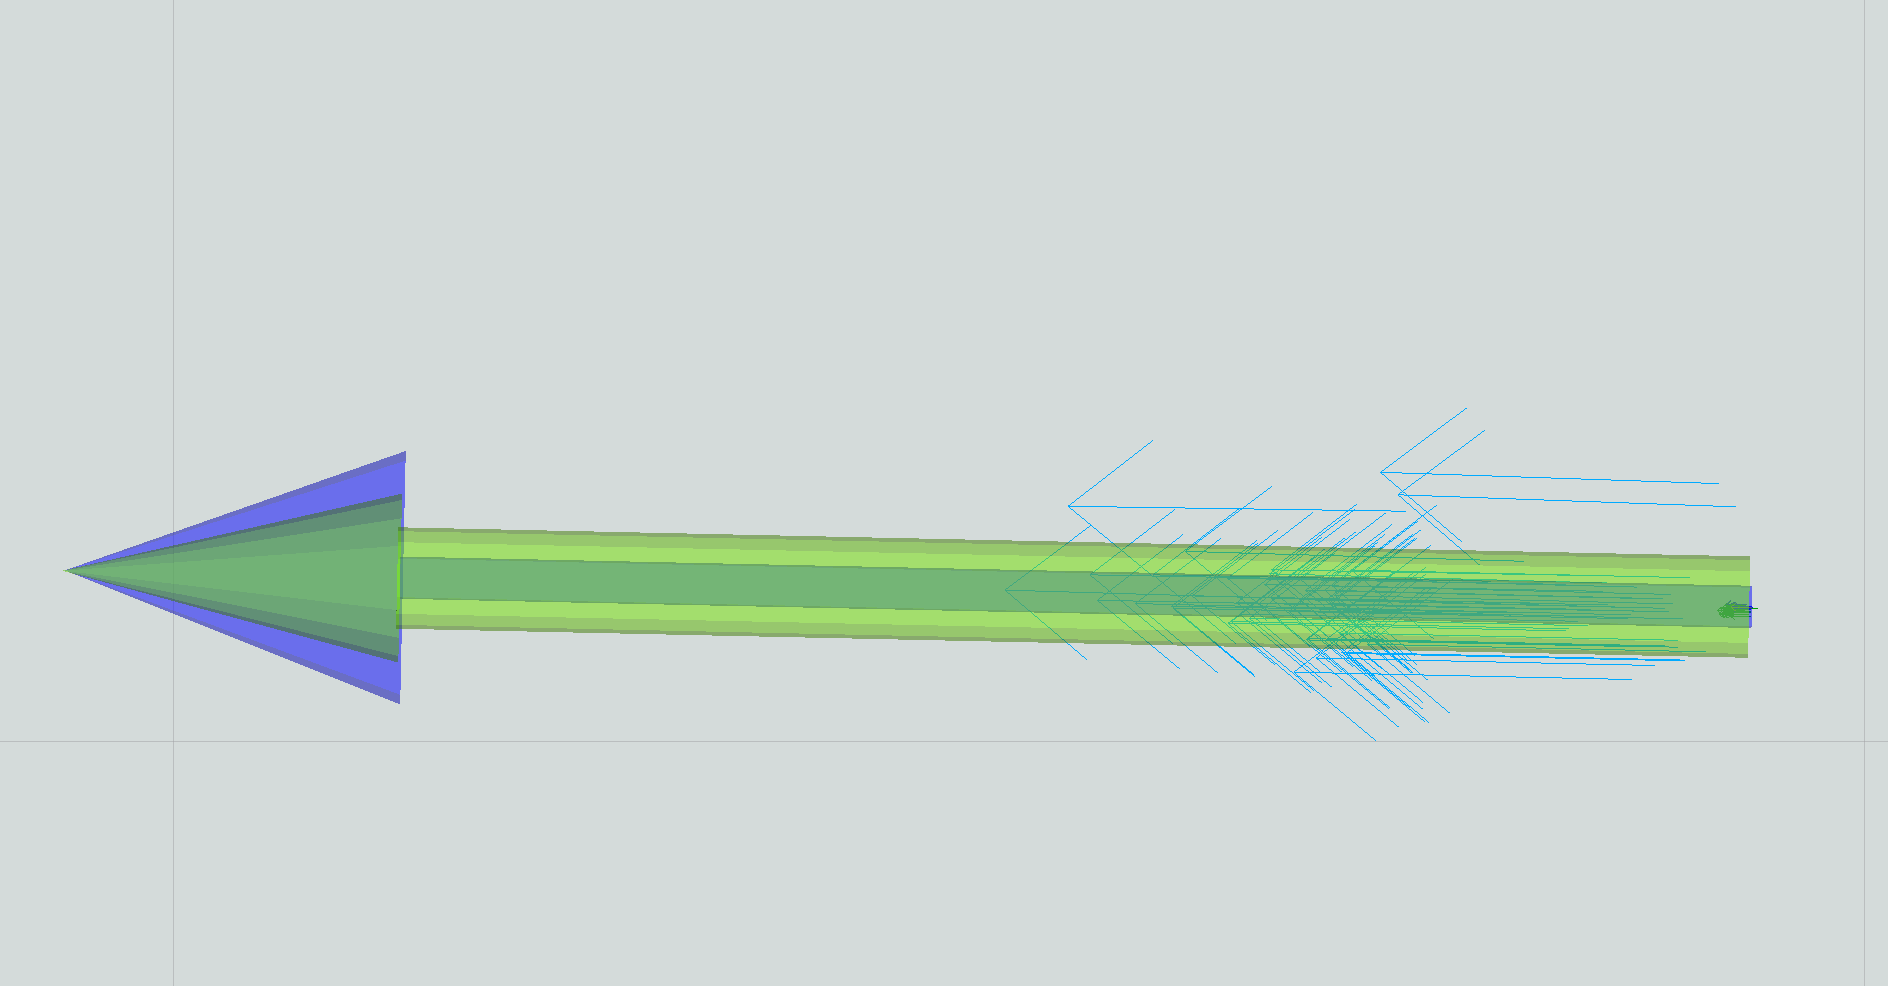
\includegraphics[width=0.4\textwidth]{localization-system-evaluation/tests-3dof/initial_pose_estimation/jarvis-initial-pose-estimation-sift-fpfh-ransac-gicp-2}
	\caption{Initial pose estimation distribution in Jarvis environment}
	\label{fig:localization-system-evaluation_jarvis-initial-pose-estimation-sift-fpfh-ransac-gicp-2}
\end{figure}




\subsection{Translation and rotation errors}

By analyzing \cref{tab:localization-system-evaluation_3-dof-results,tab:localization-system-evaluation_3-dof-results-odometry-amcl} it can be seen that the proposed 3 \gls{dof} localization system can achieve pose tracking with less than 1 cm in translation error and less than 1 degree in rotation error.

As expected, the tests at lower velocities had less mean error than the ones at higher speeds while requiring slightly less computation time. Also, the tests on the Jarvis robot had more mean error than the corresponding simulator tests. This is due to laser scan deformation that couldn't be simulated and also because the simulators were only able to add Gaussian noise to the laser measurements. To compensate the simulators limitations, the error in odometry and laser measurements in simulation was deliberately higher than the expected values for the physical platforms. This explains why the localization system needed more time to perform the pose estimations in the simulator tests. It can also be seen that adding unknown objects increased the mean error and required computation time while adding dynamic objects increased these values even further (given that a moving object appears in a laser scan as a deformed version of its static shape).

Comparing the results of the tests performed with Jarvis robot  with the tests of the Pioneer robot, it can be seen that even severely reducing the laser range (from 80 to 6 meters), moving the robot in dynamic environments with large occluding objects and even when using a low resolution map (25 mm in the Pioneer tests vs 10 mm in the Jarvis tests), the localization system still managed to track the robot pose with mean translation error (17 mm) bellow the map resolution (25 mm).

These results show that the localization system can reliably achieve high accuracy pose tracking even in dynamic and challenging environments.


\subsection{Computation time}

Looking at the computation time graphs in \cref{tab:localization-system-evaluation_3-dof-results} and \cref{app:appendix-a} it can be seen that the localization system can register the point clouds very fast (between 5 and 30 milliseconds), which is more than enough to process all the incoming laser scans in real time (typically \glspl{lidar} generate scans every 100 milliseconds). Moreover, the computation time seems to be very stable, with occasional peaks due to laser deformation or varying percentage of outliers.

The global computation time is mostly associated with the point cloud registration stage, while the rest of it is due to normal estimation and point cloud preprocessing algorithms.



%
%\section{6 \glsentrytext{dof} localization system tests}
%
%\subsection{Overview}
%
%FF.
%
%\subsection{Results}
%
%FF.
%
%\subsection{Results discussion}
%
%FF.
